% !TEX root = ../main.tex
\chapter{Dynamikk}
\label{Chapter:dynamikk}
\chaptersubtitle{— årsaken til bevegelse}
\intro{Så langt har vi tatt bevegelse for gitt, og studert hvordan legemer beveger seg. Vi har ikke spurt oss hvorfor de beveger seg, eller hva som er årsaken til bevegelsen. I dette kapitlet skal vi jobbe med den \textit{mekaniske årsaken til bevegelse.} Da blir begrep som \textit{bevegelsesmengde} og ikke minst \textit{kraft} viktige.}
\spm{}{%
\item ``May the force be with you!´´ Takk, men... hva er egentlig en kraft (``force'' på engelsk)?
\item Hvorfor er det verre å krasje med en buss som kjører i 5 km/t enn en flue som flyr i 5 km/t?
}
\section{Bevegelsesmengde}
Når man gjennom middelalderen studerte bevegelse, kom man fram til at produktet av legemets masse og dets fart er en viktig størrelse.
\[p = m \cdot v\]
I dag kaller vi denne størrelsen for \textit{bevegelsesmengde}, og det er rett og slett det det er: et mål på mengden bevegelse. Begrepet tar sikte på å forklare to aspekter ved bevegelse. For det første så er det mye bevegelse når farten er stor. For det andre er det mer bevegelse når massen er stor. En bøffel som løper på savannen har bevegelse. Men 100 bøfler som løper i samme retning utgjør mer bevegelse. Og intuisjonen viser seg å være riktig: Det er hensiktsmessig å ta med både masse og fart i definisjonen av det vi skal kalle bevegelsesmengde.

I tillegg har bevegelse retning, så i den formelle definisjonen av bevegelsesmengde er det viktig å huske på at det er en vektor, og ikke en skalar størrelse. Det betyr at bevegelsesmengde har både størrelse og retning.

\defn{Bevegelsesmengde}{
Bevegelsesmengde, $p$, er definert som produktet av et legemes masse, $m$, og dets hastighet, $v$:
\[\vec{p} = m \cdot \vec{v}\]
Enheten for bevegelsesmengde er kg·m/s.
}
Bevegelsesmengde er et viktig konsept i fysikken, spesielt i mekanikk og partikkelfysikk, fordi den er bevart i isolerte systemer. Vi kommer tilbake til dette om litt, etter at vi har definert krefter ordentlig.


\exm{Ishockey-puck}{%
En ishockey-puck har masse $m = \SI{170}{\gram}$ og slås slik at den oppnår farten $v = \SI{40}{\metre\per\second}$.
Hva er bevegelsesmengden til pucken?
}

\svar{%
\noindent
Vi gjør om massen til kilogram:
\[
    m = \SI{170}{\gram} = \SI{0.170}{\kilo\gram}
\]
Deretter bruker vi definisjonen av bevegelsesmengde:
\[
    p = m \cdot v = \SI{0.170}{\kilo\gram} \cdot \SI{40}{\metre\per\second}
    = \doubleunderline{\SI{6.8}{\kilo\gram\metre\per\second}}
\]
}

\oppgaver{Geværkule og bil}{k4oppg1}{%
%
En typisk geværkule har masse $m_k = \SI{10}{\gram}$ og forlater løpet med fart $v_k = \SI{900}{\metre\per\second}$.
En bil har masse $m_b = \SI{1500}{\kilo\gram}$.
\begin{enumerate}[a)]
    \item Finn bevegelsesmengden til geværkula.
    \item Hvor fort må bilen kjøre for å ha nøyaktig samme bevegelsesmengde som kula?
          Gi svaret i både \si{\metre\per\second} og \si{\kilo\metre\per\hour}.
\end{enumerate}
%
}

\section{Newtons lover og kraft-begrepet}
\begin{wrapfigure}[6]{r}[1.5cm]{3.6cm}
\vspace{-\baselineskip}%
\rotatebox{15}{\href{https://youtu.be/i6viZK9dZxI?si=yZVoGRbTlBLacl2F}{%
\begin{tikzpicture}[inner sep=0pt]
\node[anchor=south west] (thumb) at (0,0) {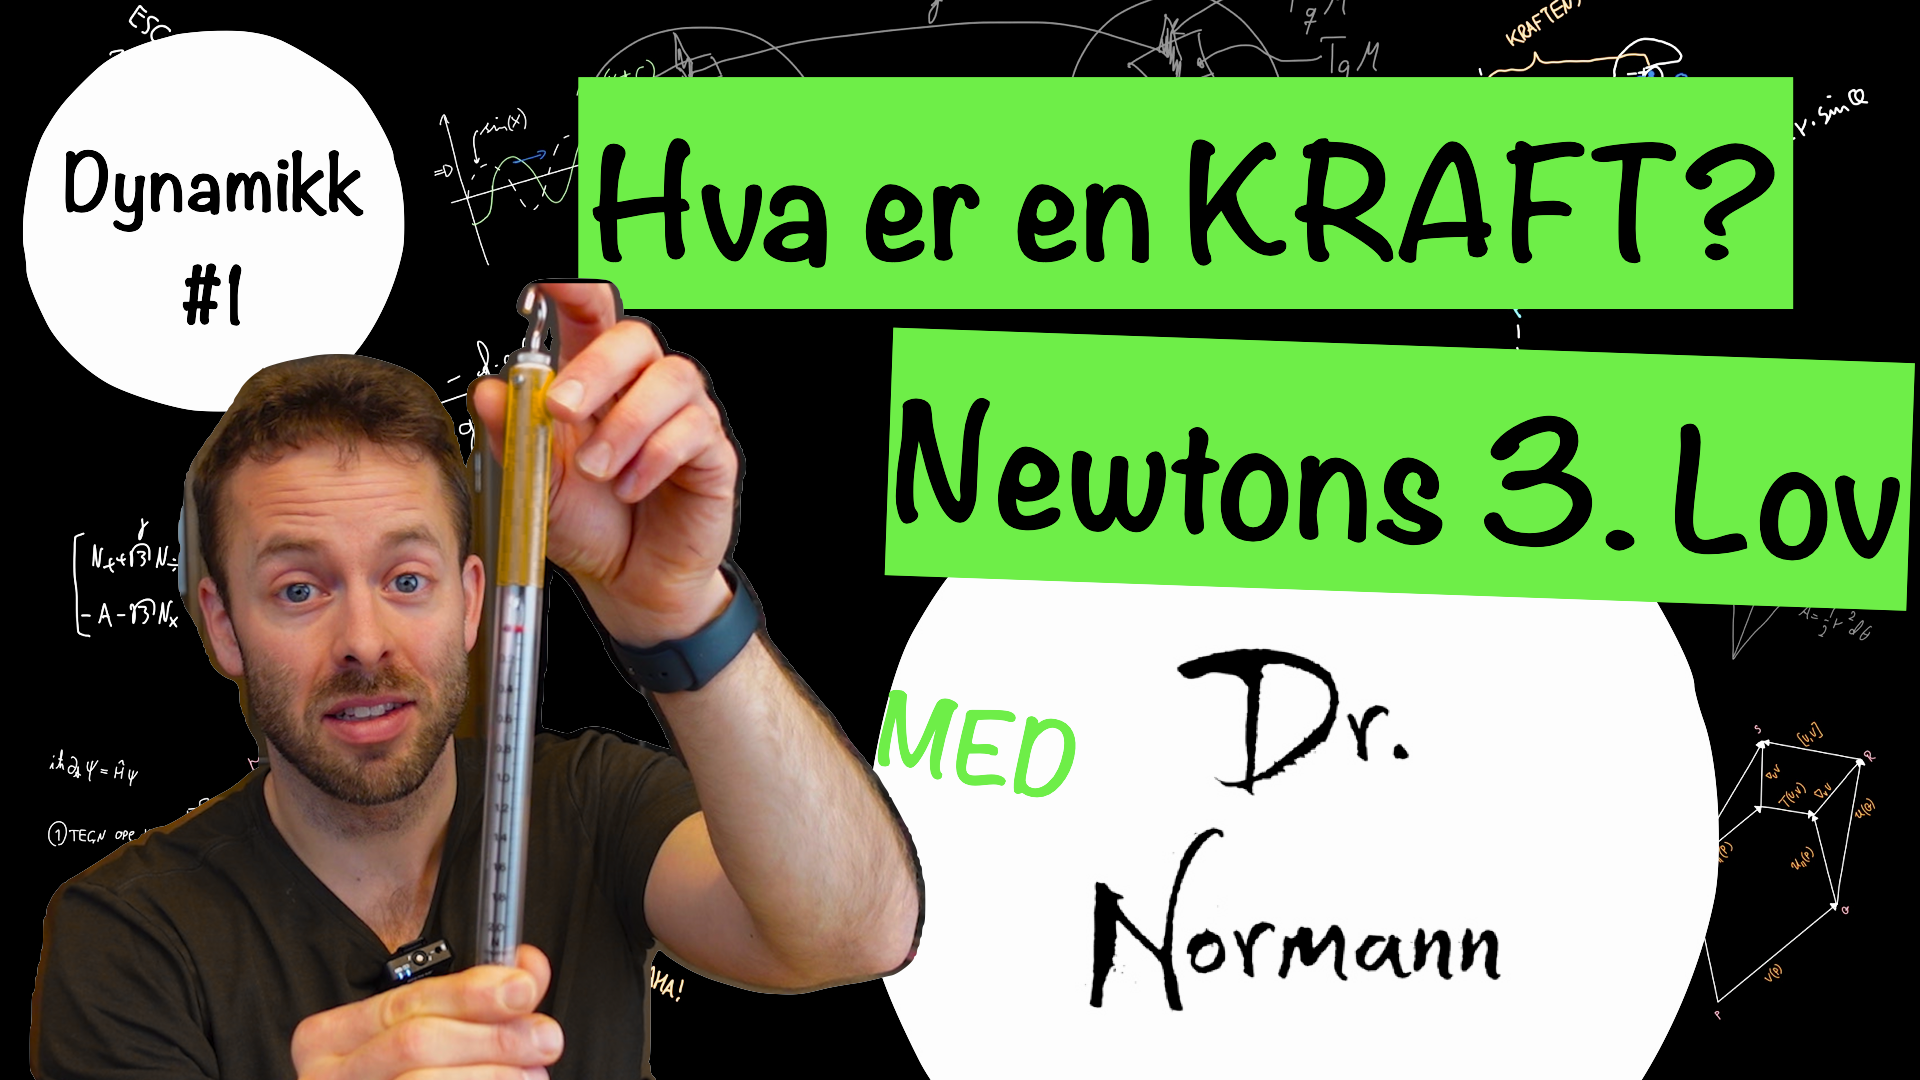
\includegraphics[width=3.6cm]{Images/YouTubeLenker/YT_NewtonsTredjeLov.png}};
\node[anchor=north west] at (thumb.south west) {
\includegraphics[width=1.2cm]{Images/YouTubeLenker/Icon.png}};
\end{tikzpicture}%
}}%
\end{wrapfigure}
Se for deg en ishockey-puck ute på isen. Hva skal til for å endre bevegelsen til pucken? Jo, da må pucken interagere med et annet legeme. Så langt har vi brukt begrep som \textit{legeme} og \textit{objekt} om hverandre. La oss være litt mer presise:
\defn{Legeme}{%
Et legeme er et objekt med masse og posisjon. Massen $m$ måles i kg (kilogram), og posisjonen $\vec{r}$ måles i meter (m).
}
Dette kan være alt fra en liten partikkel til en stor planet. Alle legemer kan derfor erverve bevegelsesmengde, så lenge de kan interagere med andre legemer. Legemer er brikkene i spillet vi kaller \textit{dynamikk}. Dette spillet har videre noen regler for hvordan brikkene, altså legemene, kan interagere. Interaksjon mellom legemer kalles i fysikken for \text{krefter}. Vi sier at \textit{krefter} er \textit{vekselvirkning mellom legemer}. Og som i all interaksjon så er den ikke ensidig. Dersom legeme A virker på legeme B, så virker legeme B på legeme A. Det som kanskje ikke er like opplagt, er at legemene virker like mye på hverandre. Det vil si at kraften som legeme A utøver på legeme B, er like stor som kraften som legeme B utøver på legeme A, bare i motsatt retning. Dette kalles Newtons tredje lov, og vi skal tenke på den som en av tre krav som totalt sett gjør \textit{kraft}-begrepet veldefinert si fysikken.

\defn{Kraft som vekselvirkning}{%
En kraft er en vekselvirkning mellom legemer. Krefter opptrer derfor alltid i par, slik at dersom legeme $A$ virker på legeme $B$ med en kraft $\vec{F}$, så virker legeme $B$ på legeme $A$ med en kraft $\vec{F}^\prime$. Videre er disse to kreftene like store, men motsatt rettet;
\[\vec{F}=-\vec{F}^\prime\qquad \textbf{(Newtons 3. lov)}.\]
Enheten for kraft er Newton (N), til ære for Isaac Newton, som var den første til å formulere en systematisk teori for krefter og bevegelse.
}

\begin{figure}[ht!]
\centering
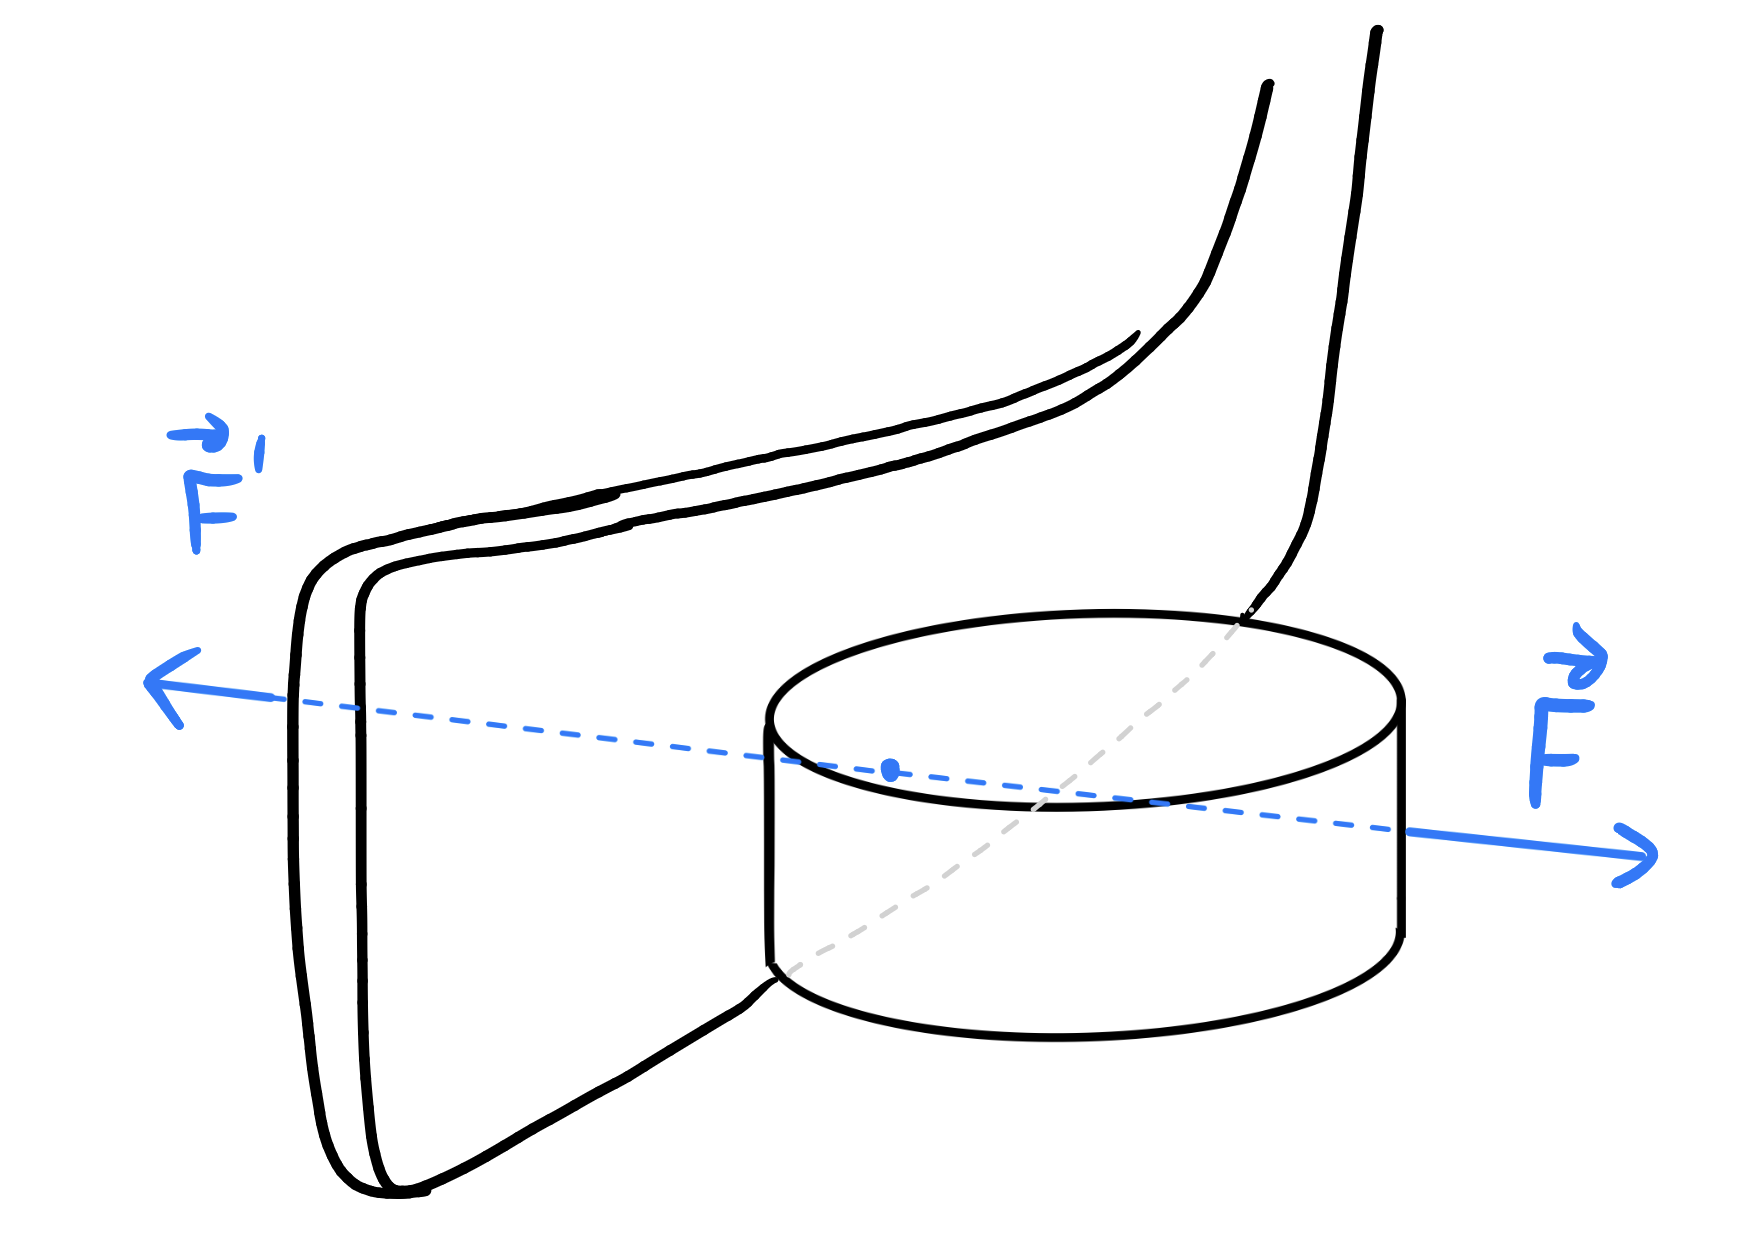
\includegraphics[width=0.6\textwidth]{Images/Kapittel4:Dynamikk/Kraft_motkraft.png}
\caption{Kraft er vekselvirkning mellom to legemer, og krefter opptrer derfor alltid i par: kraft og motkraft, som virker på hvert sitt legeme. Disse kreftene er alltid like store og motsatt rettet.}
\label{fig:kraft_motkraft}
\end{figure}

\begin{wrapfigure}[6]{r}[1.5cm]{3.6cm}
\vspace{-\baselineskip}%
\rotatebox{-15}{\href{https://youtu.be/4T2FuMioFfE?si=CVrL4VSPD85bAIcg}{%
\begin{tikzpicture}[inner sep=0pt]
\node[anchor=south west] (thumb) at (0,0) {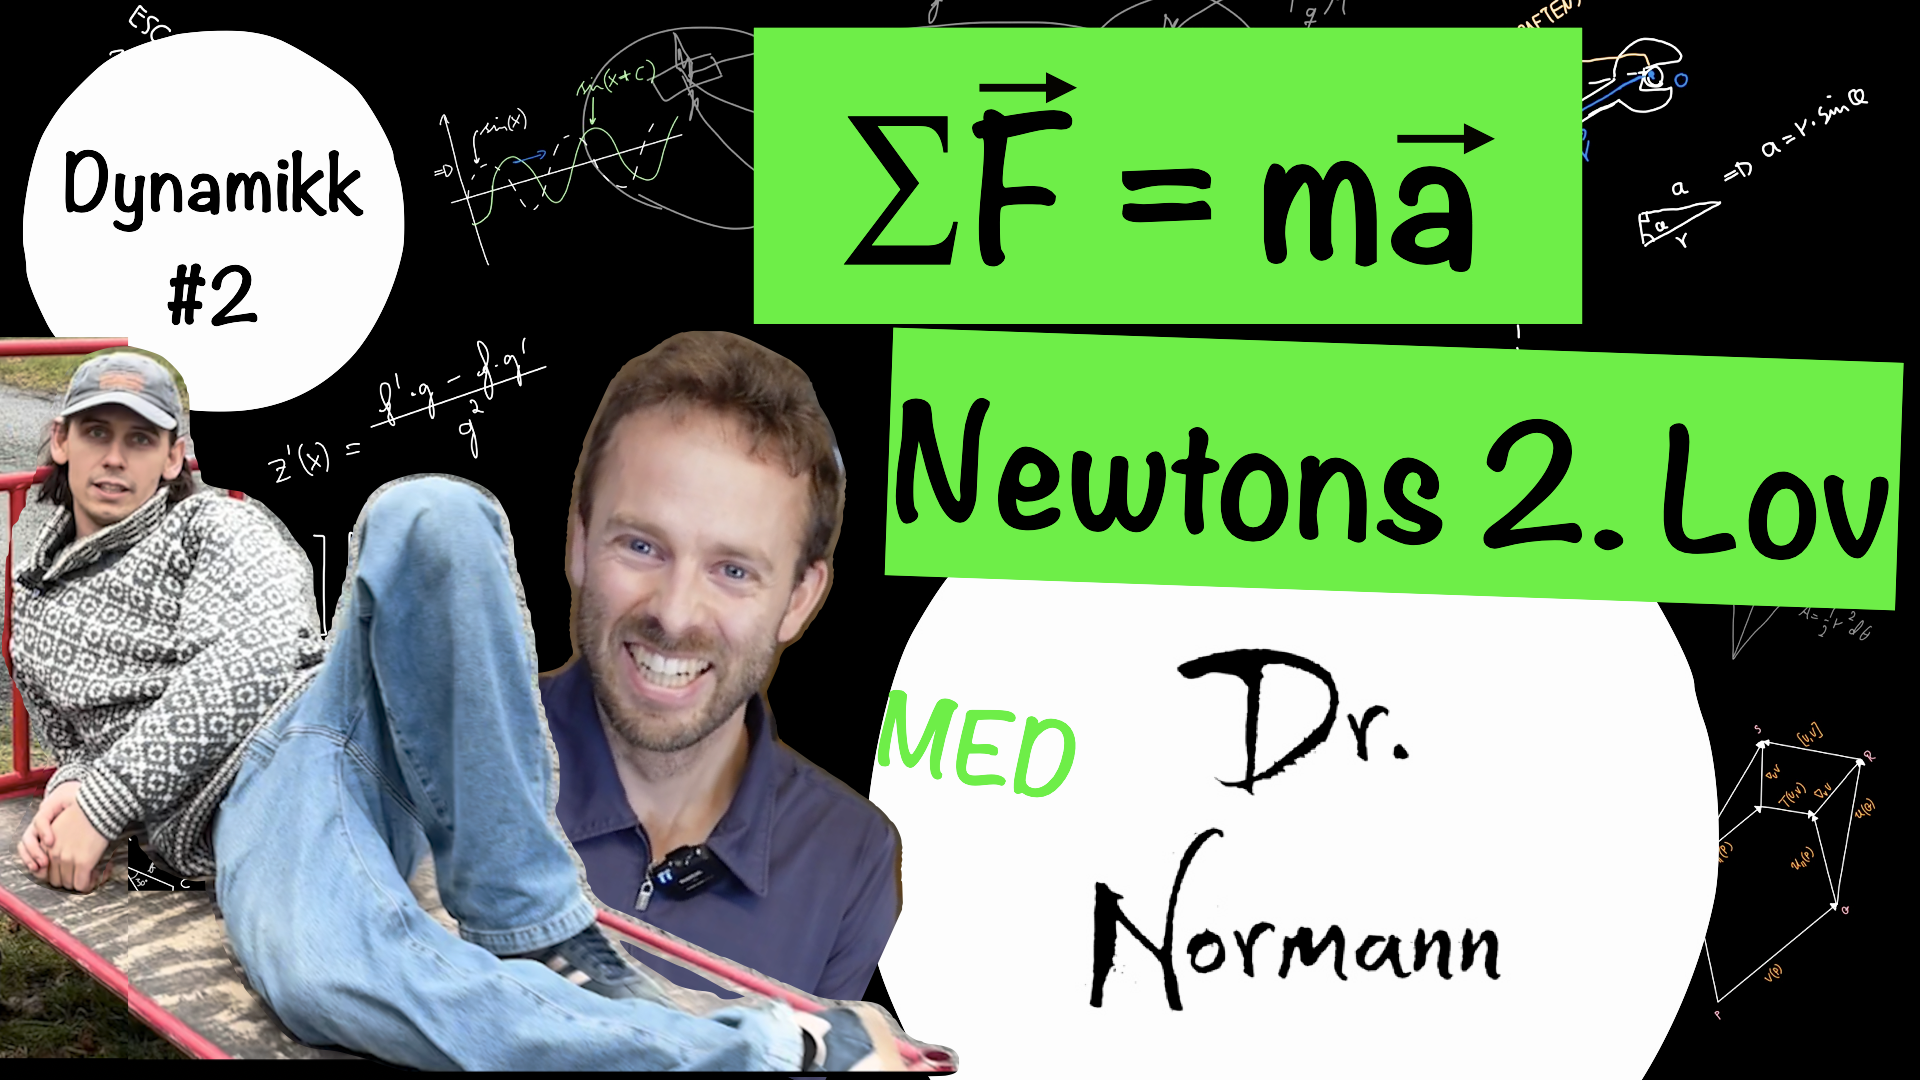
\includegraphics[width=3.6cm]{Images/YouTubeLenker/YT_NewtonsAndreLov.png}};
\node[anchor=north west] at (thumb.south west) {
\includegraphics[width=1.2cm]{Images/YouTubeLenker/Icon.png}};
\end{tikzpicture}%
}}%
\end{wrapfigure}
Videre kan vi spørre hva som skjer når legemer vekselvirker, altså når det virker krefter mellom legemene. Pucken i interaksjon med hockeykøllen er et eksempel, og her ser vi tydelig hva som kan skje: pucken på isen får sin bevegelse endret; altså endret bevegelsesmengde. La oss bruke begrepet bevegelsesmengde for å beskrive denne endringen. La oss si at pucken først hadde en bevegelsesmengde
\(\vec{p}_1=m\vec{v}_1\). Så dytter du den med hockey-køllen en tid $\Delta t$, slik at pucken endrer retning og fart. Da virker det krefter mellom hockeykøllen og pucken i dette tidsrommet. Etter interaksjonen har pucken bevegelsesmengde \(\vec{p}_2=m\vec{v}_2\). Det er ikke sikkert du dytter like hardt på pucken hele tiden gjennom interaksjonen, og det begrepet som viser seg å ha størst nytte er derfor endringen av bevegelsesmengde \textit{per tid}. Først finner vi at  $\Delta \vec{p}$:
\[\Delta \vec{p} = \vec{p}_2 - \vec{p}_1=m(\vec{v}_2 - \vec{v}_1)=m\Delta\vec{v}.\]
Gjennomsnittsendrignen \textit{per tid} må derfor være 
\[\frac{\Delta \vec{p}}{\Delta t} = m\frac{\Delta\vec{v}}{\Delta t}=m\vec{a}.\]
Denne endringen skyldes vekselvirkning mellom legemene (kølla dytter pucken, og pucken dytter tilbake mot kølla), altså \textit{krefter}. Summen av krefter som har virket på pucken i løpet av tidsrommet $\Delta t$ må nå være gitt ved
\[\sum\vec{F}=\frac{\Delta \vec{p}}{\Delta t}= m\vec{a}.\]
Kraft som årsak til hastighetsendring er oppsumert i det som er kjent som Newtons 2. lov.
\defn{Kraft som endring av bevegelse}{%}
Dersom et legeme blir påvirket av én eller flere krefter vil legemet akselerere i retning av  resultant-kraften $\sum\vec{F};$
\begin{align}
\Sigma\vec{F} = m \cdot\vec{a}\qquad \textbf{(Newtons 2. lov)}.
\end{align}
Fra denne sammenhengen ser vi at enheten for kraft, Newton (N) kan uttrykkes som \[\textrm{N}=\textrm{kg}\cdot\frac{\textrm{m}}{\textrm{s}^2}\]
}
Matematisk sett så beskrives altså krefter som vektorer. Derfor bruker vi pil over symbolet for kraft; $\vec{F},$ mens sylbolet \textit{uten} vektortegn, altså i dette tilfellet $F$, betegner størrelsen på kraften.

Tilslutt er det verdt å skrive ned en lovmessighet som gjelder et legeme hvor summen av krefter som virker på legemet er null. Et eksempel kan være en stige mot en vegg, eller en person som sitter og ser ut vinduet på et tog som suser avsted med konstant fart. Summen av påvirkning på stigen er slik at stigen står i ro. Personen i toget påvirkes også av krefter, men på en slik måte at det ikke er noen hastigehtsendring. Men går det an å ha akselerasjon dersom $\sum\vec{F}=0$? Vel, fra Newtons 2. lov ser vi at dersom $\sum\vec{F}=0$ så må vi enten ha $m\to 0$ eller $\vec{a}\to 0$. Så dersom vi krever $\vec{a}\neq 0$ så står vi igjen med $m\to 0$. Kan det hende at massen forsvinner når kreftene forsvinner? 

\begin{wrapfigure}[6]{r}[1.5cm]{3.6cm}
\vspace{-\baselineskip}%
\rotatebox{15}{\href{https://youtu.be/Co4H1ipYS9s?si=fcG3V5R-5l3F1cds}{%
\begin{tikzpicture}[inner sep=0pt]
\node[anchor=south west] (thumb) at (0,0) {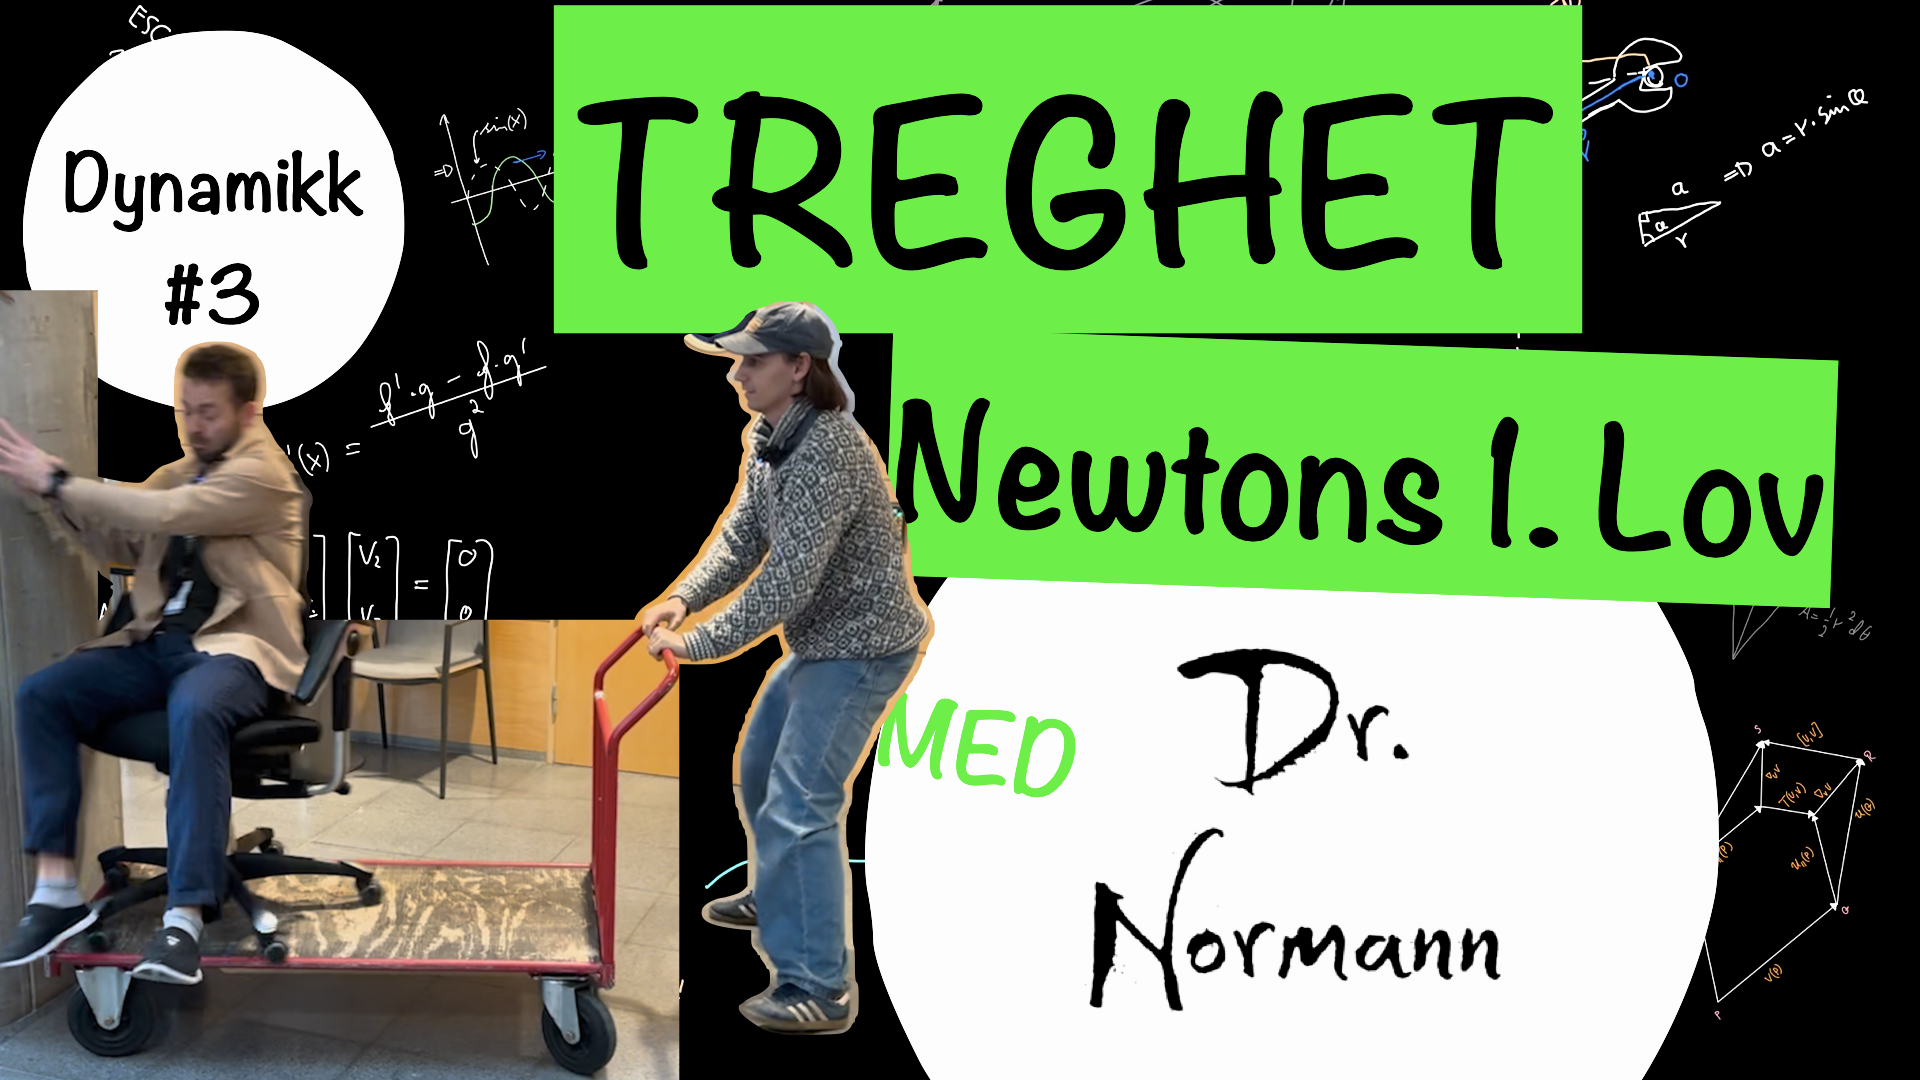
\includegraphics[width=3.6cm]{Images/YouTubeLenker/YT_NewtonsForsteLov.png}};
\node[anchor=north west] at (thumb.south west) {
\includegraphics[width=1.2cm]{Images/YouTubeLenker/Icon.png}};
\end{tikzpicture}%
}}%
\end{wrapfigure}
Hvordan sammenhengen mellom bevegelse og vekselvirkning egentlig er, tok det lang tid å foredle. Aristoteles trodde for eksempel at et legeme hadde en slags indre drivkraft. En stein som kastes og forlater hånden ville derfor fortsette i en rett linje oppover, før den plutselig falt mot bakken. Legemer hadde altså en iboende slags kraft. Det var midt imot slikt gammelt tankegods at Newton formulerte sine lover. Nei, sa Newton, bevegelse er ikke forårsaket av en iboende kraft i materien. Snarere er det slik at alle legemer vil beholde den bevegelsen de har såfremt det virker ytre krefter som forstyrrer bevegelsen. Legemers evne til å beholde bevegelsen sin, kaller vi \textit{treghet}. Og dette er det vi i dagligtale kaller \textit{masse}. I motsetning til kraft, så er tregheten (altså massen) en iboende egenskap ved materie. Newton sier altså at $m\to0$ ikke er en gyldig løsning. Legemer beholder sin treghet, eller masse. La oss formulere dette som en egen lov. Dersom summen av krefter er null, må det derfor være slik at også akselerasjonen blir null, slik det beskrives i Newtons 1. lov:

\defn{Krefter og treghet}{%
Alle legemer har en iboende treghet, kalt \textbf{masse}, som gjør at bevegelsen beholdes så lenge det ikke virker krefter på legemet:
\begin{align}
\Sigma\vec{F} = 0\Leftrightarrow v=\text{konst.}\qquad \textbf{(Newtons 1. lov)}.
\end{align}}
Konstant bevegelse krever derfor ingen mekanisk årsak (krefter).Endring i bevegelse må derimot forklares. Forklaringen er alltid at det har virket krefter. Mekanikk handler derfor i stor grad om å finne ut hvilke krefter som virker på et system, for deretter å analysere hva slags bevegelse disse kreftene eventuelt vil forårsake.




\section{Krefter i dagliglivet}
I dette avsnittet viser vi noen eksempler på krefter som du møter i hverdagen.
\tanke{}{%
Hvordan måler vi krefter?}
For å måle og sammenlikne krefter med hverandre bruker vi noe som kalles et \textit{Newtonmeter}. Det er rett og slett en fjær som presses sammen i et rør. Jo mer den presses sammen, jo større er krafta som trykker på fjæra. Så... la oss starte med å studere nettopp kraften fra en spiralfjær.

\subsection{Kraft fra spiralfjær}
Tenk på en spiralfjær. Når den er uspennt, hviler den i sin naturlige lengde — vi kaller dette \textit{likevektsposisjonen}. Presser du fjæra sammen (eller drar den ut), vil den forsøke å sprette tilbake. Jo mer du presser, jo sterkere er kraften som prøver å rette den ut igjen.

La $\vec{x}$ betegne forflytningen til den ene enden av fjæra fra likevektsposisjonen. Da er fjærkraften gitt ved Hookes lov:

\defn{Hookes lov}{%
Kraften fra en fjær på det den er festet til er proporsjonal med avviket $\vec{x}$ fra likevektsposisjonen:
\[
    \vec{F} = -k\vec{x}
\]
Her er $k > 0$ \textit{fjærkonstanten} (enhet: \si{\newton\per\metre}), og $\vec{x}$ er forflytningen fra likevekt. Minustegnet viser at kraften alltid peker \textit{mot} likevekt — uansett om fjæra er presset sammen eller strukket ut.
}

\noindent
\begin{minipage}[t]{0.50\linewidth}
\vspace{0pt}
Figur~\ref{fig:hooke} viser en fjær som er presset sammen. Vi definerer positiv $x$-retning mot høyre. Fjæra presses slik at avviket fra likevekt er $\vec{x}$ (peker mot venstre, altså $x < 0$). Da er fjærkraften
\[
    \vec{F} = -k\vec{x},
\]
som peker mot høyre — tilbake mot likevekt. Stivheten til fjæra bestemmes av fjærkonstanten $k$: en stiv fjær (stor $k$) gir stor kraft selv ved lite avvik, mens en myk fjær (liten $k$) gir liten kraft.
\end{minipage}%
\hfill
\begin{minipage}[t]{0.47\linewidth}
\vspace{0pt}
\centering
\begin{tikzpicture}[font=\small, scale=1.0]
  % Wall
  \fill[black!15] (-0.35,-0.85) rectangle (0,0.85);
  \draw[very thick] (0,-0.85) -- (0,0.85);
  \foreach \y in {-0.70,-0.45,-0.20,0.05,0.30,0.55,0.70} {
    \draw[black!40, thin] (0,\y) -- (-0.28,\y+0.22);
  }
  % Spring (compressed zigzag, x=0 to x=2.6)
  \draw[line width=1.2pt, headCol!70!black]
    (0,0)
    -- (0.20, 0)
    -- (0.35, 0.38) -- (0.55,-0.38)
    -- (0.75, 0.38) -- (0.95,-0.38)
    -- (1.15, 0.38) -- (1.35,-0.38)
    -- (1.55, 0.38) -- (1.75,-0.38)
    -- (1.95, 0.38) -- (2.15,-0.38)
    -- (2.35, 0.38) -- (2.50, 0)
    -- (2.70, 0);
  % Block
  \fill[headCol!18] (2.70,-0.45) rectangle (3.40,0.45);
  \draw[headCol!65!black, thick] (2.70,-0.45) rectangle (3.40,0.45);
  \node at (3.05, 0) {$m$};
  % Equilibrium dashed line
  \draw[dashed, black!50, semithick] (4.10,-0.75) -- (4.10,0.75);
  \node[black!55, font=\scriptsize, above] at (4.10,0.75) {likevekt};
  % x arrow: from current block pos to equilibrium (x < 0, arrow points left)
  \draw[-{Stealth[length=7pt,width=5pt]}, black!65, semithick]
    (4.10,-0.68) -- (3.40,-0.68);
  \node[black!65, font=\scriptsize, below=2pt] at (3.75,-0.68) {$\vec{x}$};
  % F arrow: restoring force points right
  \draw[-{Stealth[length=11pt,width=7pt]}, line width=2.5pt, defscol]
    (3.40,0) -- (4.55,0);
  \node[right=3pt, defscol, font=\normalsize\bfseries] at (4.55,0) {$\vec{F}$};
  % Floor
  \draw[black!30, thin] (-0.35,-0.88) -- (5.0,-0.88);
\end{tikzpicture}
\captionof{figure}{Fjær trykket sammen. Avviket $\vec{x}$ peker mot venstre (fra likevekt til klossen), og fjærkraften $\vec{F}=-k\vec{x}$ peker mot høyre — tilbake mot likevekt.}
\label{fig:hooke}
\end{minipage}

\medskip

\exm{Komprimert fjær}{%
En spiralfjær har fjærkonstant $k = \SI{250}{\newton\per\metre}$. Den trykkes \SI{6.0}{\centi\metre} sammen fra likevektsposisjonen.
Hva er størrelsen på fjærkraften?
}

\svar{%
\noindent
Avviket fra likevekt er $x = \SI{6.0}{\centi\metre} = \SI{0.060}{\metre}$.
Hookes lov gir størrelsen på kraften:
\[
    F = k \cdot |x| = \SI{250}{\newton\per\metre} \cdot \SI{0.060}{\metre}
    = \doubleunderline{\SI{15}{\newton}}
\]
Kraften peker vekk fra veggen — tilbake mot likevektsposisjonen.
}

\oppgaver{Finn fjærkonstanten}{k4oppg2}{%
%
Du fester et lodd til en vertikal fjær og måler at fjæra strekkes \SI{12}{\centi\metre} når loddet har masse $m = \SI{250}{\gram}$.
\begin{enumerate}[a)]
    \item Hva er fjærkonstanten $k$? (Hint: når fjæra er i ro, er fjærkraften lik tyngdekraften på loddet.)
    \item Hvor mye strekkes fjæra om du bytter til et lodd med masse $m = \SI{400}{\gram}$?
\end{enumerate}
%
}

\subsection{Tyngdekraft}
\noindent
Tyngdekraften $\vec{G}$ er kraften jorda trekker et legeme mot sitt sentrum med. Størrelsen avhenger av legemets masse $m$ og hvor langt unna jordas sentrum vi er. Men på jordoverflaten viser det seg at tyngdekraften er 
\[
    \vec{G} = m\vec{\mathrm{g}},
\]
hvor $\mathrm{g}\approx \SI{9.81}{\metre\per\second\squared}$. Vi ser altså at tyngdekraften er proporsjonal med massen $m$. Dette er spesielt. For se nå for deg et legeme som faller mot jorda, kun under påvirkning av tyngdekraften. Da gir Newtons andre lov at
\begin{align*}
\sum F=ma\quad\rightarrow m\mathrm{g}=ma\\
a=\mathrm{g}=\SI{9.81}{\metre\per\second\squared}.
\end{align*}
Tyngdekraften trekker altså alle legemer mot bakken med samme akselerasjon. Dette kalles \textbf{fritt fall.}

\definecolor{dashblue}{RGB}{50,110,235}
\begin{figure}[ht!]
\centering
\begin{tikzpicture}
  \node[anchor=south west, inner sep=0] (image) at (0,0) {%
    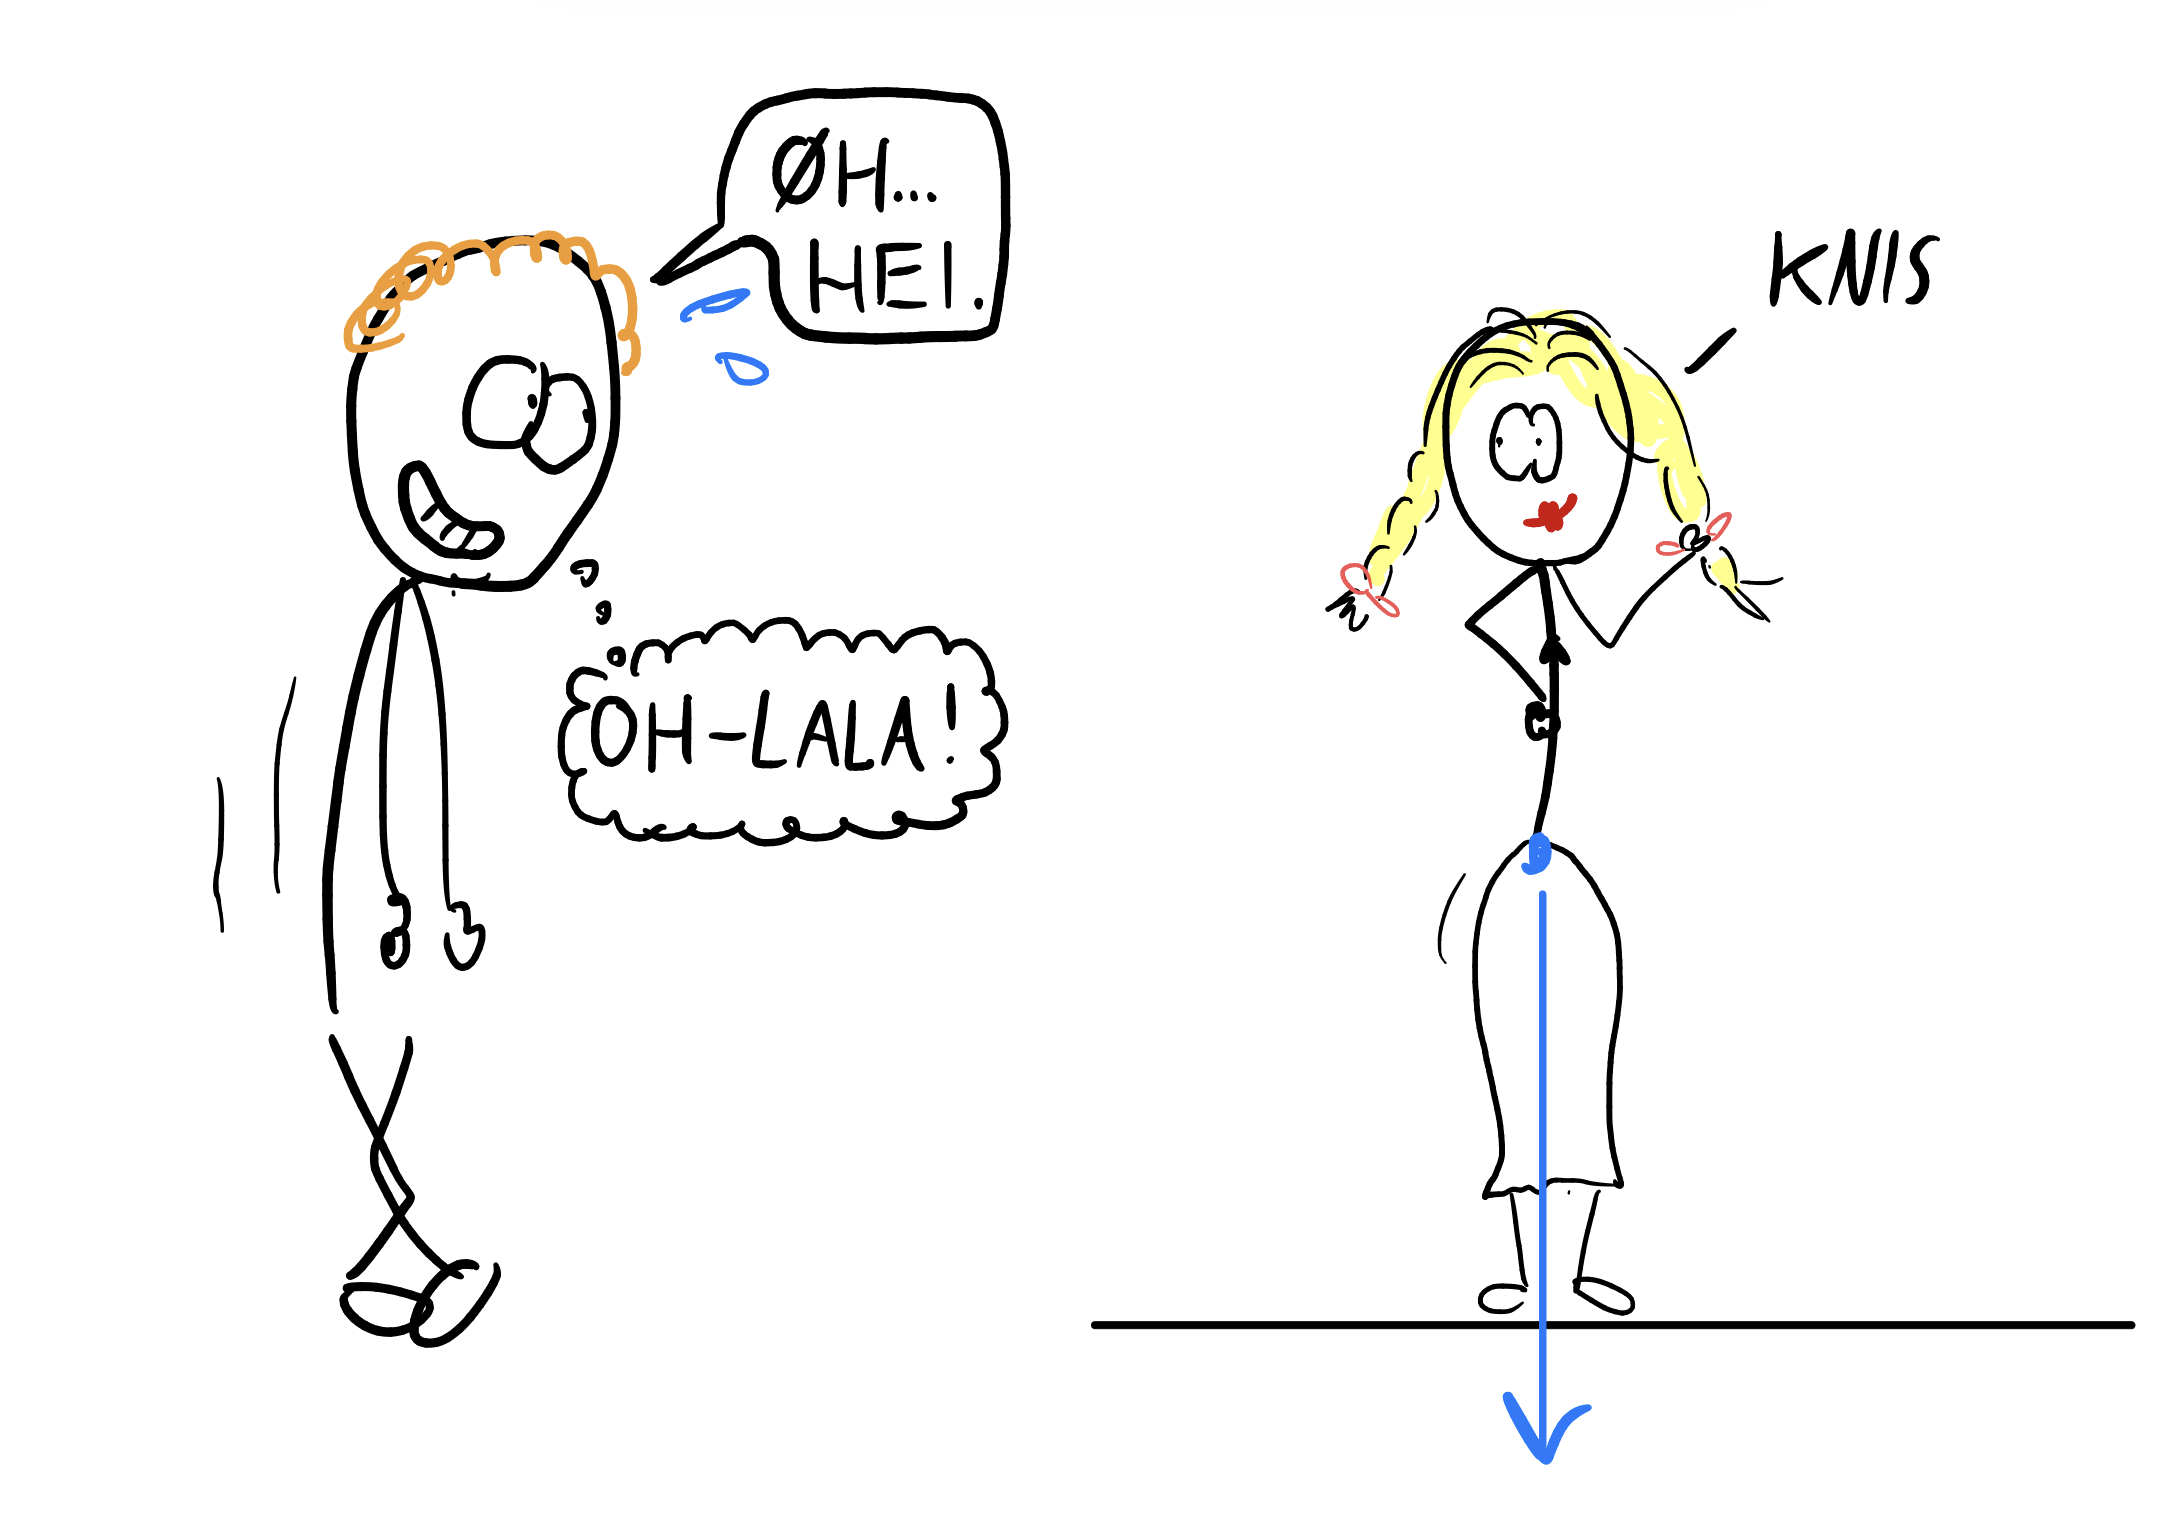
\includegraphics[width=0.85\textwidth]{Images/Kapittel4:Dynamikk/Dashman_DashLine_tyngdekraft.png}%
  };
  \begin{scope}[x={(image.south east)}, y={(image.north west)}]
    \node[anchor=north, font=\bfseries\large, text=dashblue] at (0.710, 0.035) {$G = m\mathrm{g}$};
  \end{scope}
\end{tikzpicture}
\caption{Dash-Line påvirkes av en kraft med størrelse $G=m\mathrm{g}$ fra jorda. Dashman ser ut til å være påvirket av helt andre former for tiltrekningskrefter... ;)}
\label{fig:tyngdekraft}
\end{figure}

\medskip
På overflaten av månen ville tyngdens akselerasjon vært en annen. Der har vi nemlig $\mathrm{g}_\text{måne} \approx \SI{1.62}{\metre\per\second\squared}$ — omtrent $\frac{1}{6}$ av jordas. Merk at \textit{massen} $m$ er den samme uansett hvor du befinner deg, mens \textit{tyngdekraften} $G$ varierer med stedet.
\exm{Tyngdekraft på jordoverflaten}{%
Sofie har masse $m = \SI{60}{\kilo\gram}$. Hva er tyngdekraften som virker på henne på jordoverflaten?
}

\svar{%
\noindent
Vi bruker definisjonen av tyngdekraft med $\mathrm{g} = \SI{9.81}{\metre\per\second\squared}$:
\[
    G = m \cdot \mathrm{g} = \SI{60}{\kilo\gram} \cdot \SI{9.81}{\metre\per\second\squared}
    = \doubleunderline{\SI{588.6}{\newton}}
\]
}

\oppgaver{Tyngdekraft på jord og måne}{k4oppg3}{%
%
Ola har masse $m = \SI{75}{\kilo\gram}$.
\begin{enumerate}[a)]
    \item Finn tyngdekraften på Ola på jordoverflaten ($\mathrm{g} = \SI{9.81}{\metre\per\second\squared}$).
    \item Finn tyngdekraften på Ola på månens overflate ($\mathrm{g}_\text{måne} = \SI{1.62}{\metre\per\second\squared}$).
    \item Hva er Olas masse på månen? Forklar svaret.
\end{enumerate}
%
}
\oppgaver{Fritt fall}{k4oppg4}{%
%
En hammer og en fjær slippes samtidig fra samme høyde.
\begin{enumerate}[a)]
    \item Hva tror du skjer — hvilket objekt når bakken først?
    \item Hva skjer om vi pumper vekk all lufta i rommet? Bruk det du har lært om tyngdekraft til å forklare svaret.
\end{enumerate}
%
}
\subsection{Underlagskrefter}
\noindent
\begin{minipage}[t]{0.54\linewidth}
\vspace{0pt}
Når et objekt står på et underlag så virker det krefter fra underlaget, som sørger for at objektet ikke faller gjennom. Vi dekomponerer gjerne slike \textit{underlagskrefter} $\vec{U}$ i to deler: normalkraft ($\vec{N}$) og friksjonskraft ($\vec{R}$), slik at
\[\vec{U}=\vec{N}+\vec{R}.\]
Normalkraften $\vec{N}$ virker \textit{vinkelrett} på underlaget, mens friksjonskraften $\vec{R}$ virker \textit{parallelt} med underlaget. Figur~\ref{fig:underlagskrefter} viser en fot som står på bakken — underlagskraften $\vec{U}$ kan da dekomponeres i begge disse retningene.
\end{minipage}%
\hfill
\begin{minipage}[t]{0.43\linewidth}
\vspace{0pt}
\centering
\begin{tikzpicture}
  \node[anchor=south west, inner sep=0] (image) at (0,0) {%
    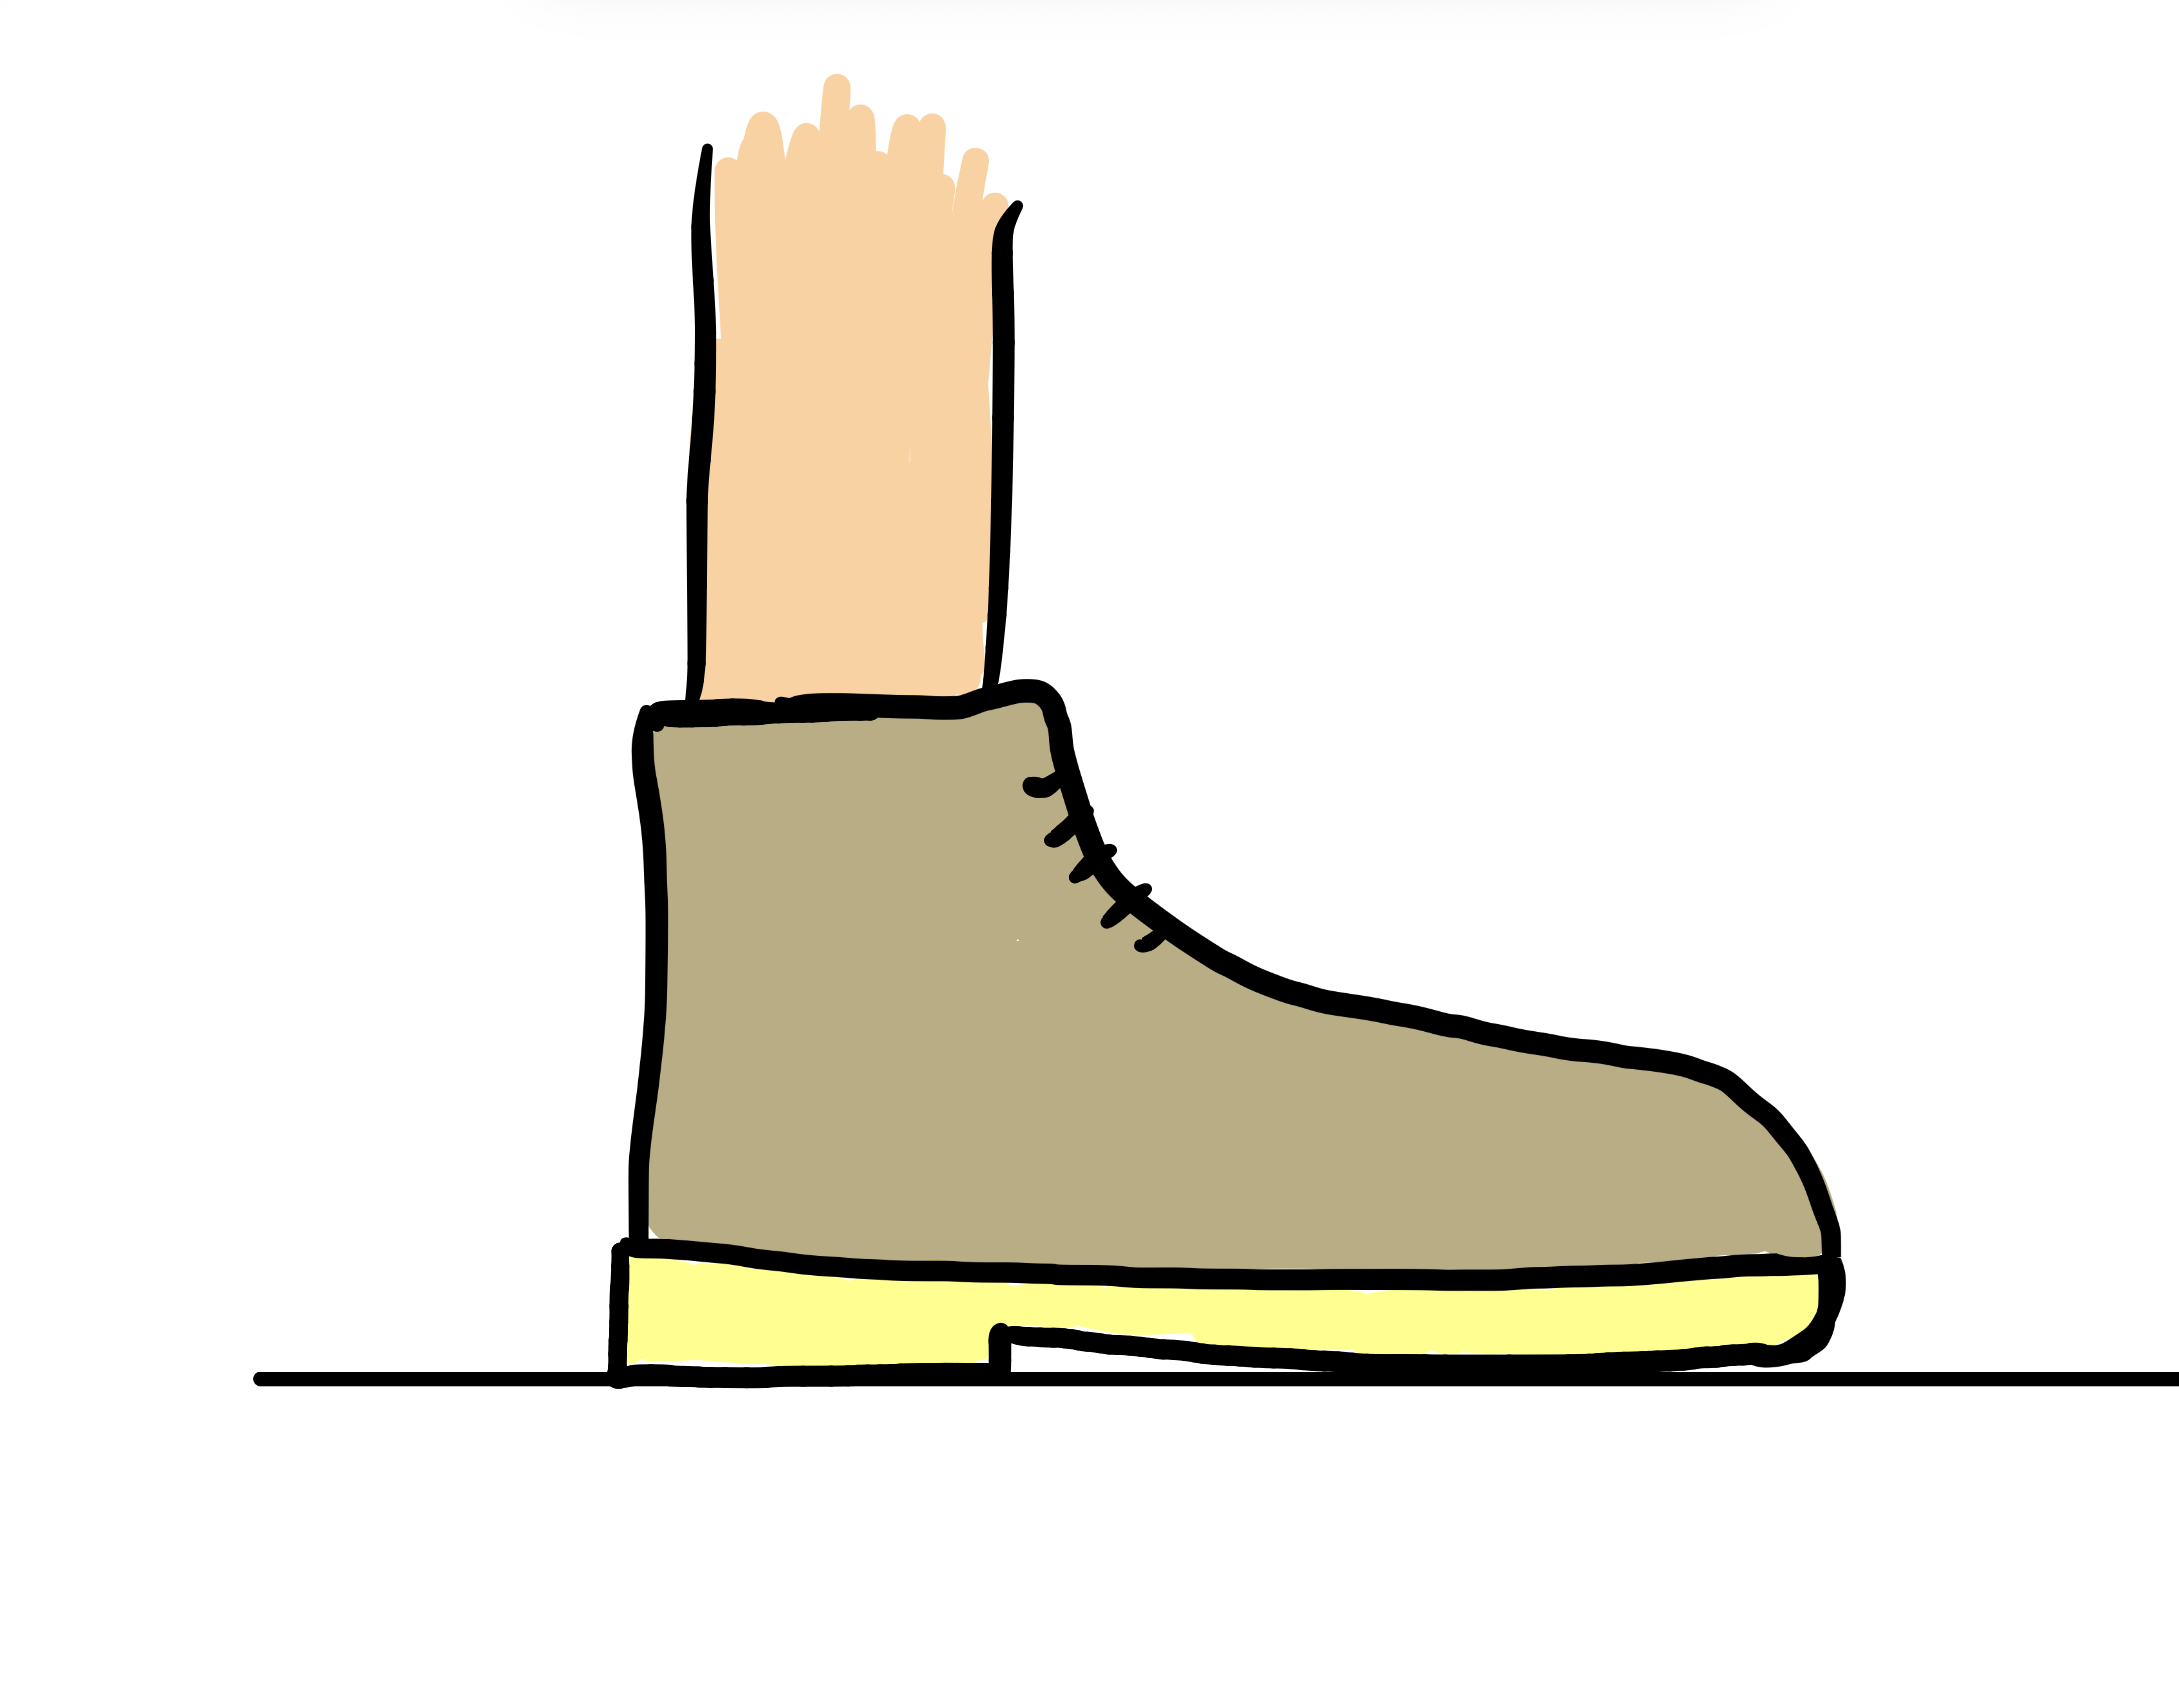
\includegraphics[width=5.6cm]{Images/Kapittel4:Dynamikk/fot_underlag_ny.png}%
  };
  \begin{scope}[x={(image.south east)}, y={(image.north west)}]
    % Contact point: under boot, between ankle and toe, at floor level
    \coordinate (P) at (0.65, 0.181);
    % N: perpendicular to floor (vertical, upward)
    \draw[-{Stealth[length=13pt,width=9pt]}, line width=2.8pt, defscol]
      (P) -- ($(P)+(0,0.32)$);
    \node[right=5pt, defscol, font=\normalsize\bfseries,
          fill=white, draw=defscol, line width=0.3pt,
          inner sep=2pt, rounded corners=1pt]
      at ($(P)+(0,0.30)$) {$\vec{N}$};
    % R: parallel to floor (horizontal, rightward)
    \draw[-{Stealth[length=13pt,width=9pt]}, line width=2.8pt, oppsumcol]
      (P) -- ($(P)+(0.19,0)$);
    \node[below=4pt, oppsumcol, font=\normalsize\bfseries,
          fill=white, draw=oppsumcol, line width=0.3pt,
          inner sep=2pt, rounded corners=1pt]
      at ($(P)+(0.095,0)$) {$\vec{R}$};
    % U: resultant diagonal
    \draw[-{Stealth[length=15pt,width=11pt]}, line width=2.8pt, black!72]
      (P) -- ($(P)+(0.19,0.32)$);
    \node[right=5pt, black!72, font=\normalsize\bfseries,
          fill=white, draw=black!50, line width=0.3pt,
          inner sep=2pt, rounded corners=1pt]
      at ($(P)+(0.19,0.32)$) {$\vec{U}$};
    % Dashed parallelogram lines
    \draw[dashed, black!40, semithick]
      ($(P)+(0,0.32)$) -- ($(P)+(0.19,0.32)$);
    \draw[dashed, black!40, semithick]
      ($(P)+(0.19,0)$) -- ($(P)+(0.19,0.32)$);
    % Right-angle marker at contact point
    \draw[black!50, thin]
      ($(P)+(0,0.025)$) -- ($(P)+(0.025,0.025)$) -- ($(P)+(0.025,0)$);
    % Dot at contact point
    \fill[black!60] (P) circle (2pt);
  \end{scope}
\end{tikzpicture}
\captionof{figure}{En fot som står på bakken. Underlagskraften $\vec{U}$ dekomponeres i normalkraften $\vec{N}$ (vinkelrett) og friksjonskraften $\vec{R}$ (parallelt med underlaget).}
\label{fig:underlagskrefter}
\end{minipage}

\medskip

La oss se nærmere på hver av disse.

\subsubsection{Normalkraft}
Normalkraften $\vec{N}$ er den delen av underlagskraften som virker \textit{vinkelrett} på underlaget (/normalt på underlaget, derav navnet). Som vi skal se i de følgende eksemplene så kan vi i mange tilfeller bruke Newtons 1. eller 2. lov til å finne størrelsen på normalkraften. 

\exm{Person i ro på flatt underlag}{%
Ola har masse $m = \SI{80}{\kilo\gram}$ og står i ro på et flatt gulv.
Hva er normalkraften som gulvet utøver på Ola?
}

\svar{%
\noindent
Siden Ola er i ro, er summen av krefter i vertikal retning null (Newtons 2. lov med $a = 0$):
\[
    \sum F_y = N - G = 0 \implies N = G = m \cdot \mathrm{g}
\]
\[
    N = \SI{80}{\kilo\gram} \cdot \SI{9.81}{\metre\per\second\squared}
    = \doubleunderline{\SI{784.8}{\newton}}
\]
Gulvet skyver Ola opp med nøyaktig like stor kraft som tyngdekraften trekker Ola ned — dette er et eksempel på Newtons 3. lov i praksis.
}
Som vi så i eksemplet over så er Normalkraften like stor og motsatt rettet i forhold til tyngdekraften når et legeme står i ro på et gulv. Slik må det nesten være, ettersom det da kun er $G$ og $N$ som virker. Likevel er ikke $N$ motkraften til $G$. 
\tanke{}{%
Hvorfor er ikke $\vec{N}$ og $\vec{G}$ et kraft-motkraft par slik som det er definert i Newtons 3. lov?}
Grunnen er enkel: Både $\vec{N}$ og $\vec{G}$ virker på samme legeme. Newtons 3. lov handler om \textit{vekselvirkning} mellom legemer, og kraft-motkraftpar virker derfor alltid på to forskjellige legemer. Det er liksom hele poenget. Derfor må vi stille oss et viktig spørsmål til.
\tanke{}{%
Hva er motkreftene til $\vec{N}$ og $\vec{G}$ i eksemplet over? På hvilke legemer virker de?}

\exm{Normalkraft i akselererende heis}{%
Kari har masse $m = \SI{70}{\kilo\gram}$ og står i en heis. Heisen akselererer oppover med $a = \SI{2.0}{\metre\per\second\squared}$.
Hva er normalkraften $\vec{N}$ som gulvet utøver på Kari?
}

\svar{%
\noindent
Vi tegner inn kreftene på Kari: tyngdekraften $\vec{G}$ peker ned og normalkraften $\vec{N}$ peker opp. Kari akselererer oppover, så vi velger oppover som positiv retning. Newtons 2. lov gir
\[
    \sum F_y = N - G = ma
\]
\[
    N = G + ma = m(\mathrm{g} + a)
    = \SI{70}{\kilo\gram} \cdot (\SI{9.81}{\metre\per\second\squared} + \SI{2.0}{\metre\per\second\squared})
    = \doubleunderline{\SI{827}{\newton}}
\]
Til sammenligning er tyngdekraften på Kari $G = \SI{70}{\kilo\gram} \cdot \SI{9.81}{\metre\per\second\squared} \approx \SI{687}{\newton}$. Normalkraften er altså større enn tyngdekraften når heisen akselererer oppover — Kari føler seg tyngre enn til vanlig.
}

\oppgaver{Normalkraft i heis — ulike situasjoner}{k4oppg5}{%
%
Ola har masse $m = \SI{80}{\kilo\gram}$ og er i en heis. Finn normalkraften $N$ i følgende tilfeller:
\begin{enumerate}[a)]
    \item Heisen bremser ned mens den beveger seg oppover, slik at $a = \SI{-3.0}{\metre\per\second\squared}$.
    \item Heisen er i fritt fall (tau røk!). Hva er $N$ da, og hva ville Ola oppleve?
\end{enumerate}
%
}

\subsubsection{Friksjonskraft}

\noindent
\begin{minipage}[t]{0.54\linewidth}
\vspace{0pt}
Friksjonskraft $\vec{R}$ er den delen av underlagskraften som virker \textit{parallelt} med kontaktflaten. Den motstår alltid relativ bevegelse mellom to overflater — eller tendensen til slik bevegelse. Figur~\ref{fig:friksjon} viser et objekt som skyves horisontalt: normalkraften $\vec{N}$ peker opp, tyngdekraften $\vec{G}$ peker ned, den påførte kraften $\vec{F}$ peker til høyre, og friksjonskraften $\vec{R}$ peker til venstre — motsatt av bevegelsesretningen.

Størrelsen på friksjonskraften avhenger av to ting: normalkraften $N$ og et tall som beskriver hvor «glatt» eller «ru» kontakten mellom overflatene er. Dette tallet kalles \textit{friksjonskoeffisienten}, og det finnes én for hvert av de to tilfellene vi nå skal studere.
\end{minipage}%
\hfill
\begin{minipage}[t]{0.43\linewidth}
\vspace{0pt}
\centering
\begin{tikzpicture}[font=\small]
  % Surface
  \fill[black!12] (-0.6,-0.38) rectangle (4.0,0);
  \draw[very thick] (-0.6,0) -- (4.0,0);
  \foreach \x in {-0.45,-0.20,...,3.85} {
    \draw[black!35, thin] (\x,0) -- (\x-0.22,-0.22);
  }
  % Block
  \fill[headCol!20] (0.80,0) rectangle (2.80,1.20);
  \draw[headCol!65!black, thick] (0.80,0) rectangle (2.80,1.20);
  \node at (2.15,0.60) {$m$};
  % N: normalkraft — angriper ved kontaktflaten (bunn av blokk), peker opp
  \draw[-{Stealth[length=11pt,width=7pt]}, line width=2.5pt, defscol]
    (1.50, 0) -- (1.50, 1.65);
  \node[left=5pt, defscol, font=\small\bfseries,
        fill=white, draw=defscol, line width=0.3pt,
        inner sep=2pt, rounded corners=1pt]
    at (1.50, 1.33) {$\vec{N}$};
  % G: tyngdekraft — angriper ved massesentrum, peker ned
  \draw[-{Stealth[length=11pt,width=7pt]}, line width=2.5pt, black!65]
    (1.80, 0.60) -- (1.80, -0.72);
  \node[right=5pt, black!65, font=\small\bfseries,
        fill=white, draw=black!50, line width=0.3pt,
        inner sep=2pt, rounded corners=1pt]
    at (1.80, -0.06) {$\vec{G}$};
  % F: påført kraft — angriper ved høyre side, peker høyre
  \draw[-{Stealth[length=11pt,width=7pt]}, line width=2.5pt, oppsumcol]
    (2.80, 0.60) -- (4.10, 0.60);
  \node[right=4pt, oppsumcol, font=\small\bfseries] at (4.10, 0.60) {$\vec{F}$};
  % R: friksjonskraft — angriper ved kontaktflaten, peker venstre
  \draw[-{Stealth[length=11pt,width=7pt]}, line width=2.5pt, red!70!black]
    (1.40, 0) -- (0.00, 0);
  \node[below=5pt, red!70!black, font=\small\bfseries,
        fill=white, draw=red!70!black, line width=0.3pt,
        inner sep=2pt, rounded corners=1pt]
    at (0.70, 0) {$\vec{R}$};
  % Prikker ved angrepspunkt
  \fill[defscol] (1.50, 0) circle (2pt);
  \fill[red!70!black] (1.40, 0) circle (2pt);
  \fill[black!55] (1.80, 0.60) circle (2pt);
\end{tikzpicture}
\captionof{figure}{Krefter på et objekt som skyves horisontalt. Friksjonskraften $\vec{R}$ virker alltid motsatt av bevegelsesretningen.}
\label{fig:friksjon}
\end{minipage}

\medskip

\defn{Friksjonskrefter}{%
Den \textbf{statiske friksjonskoeffisienten} $\mu_s$ bestemmer maksimal hvilefriksjon. Når et objekt er \textit{i ro}, tilpasser friksjonskraften seg automatisk og kan ta alle verdier opp til
\[
    R_s \leq \mu_s N.
\]
Den \textbf{kinetiske friksjonskoeffisienten} $\mu_k$ bestemmer glidefriksjonen. Når et objekt \textit{glir} langs underlaget, er friksjonskraften tilnærmet konstant:
\[
    R = \mu_k N.
\]
Begge koeffisientene er dimensjonsløse tall ($\mu > 0$) som avhenger av materialene i kontakt. Som regel er $\mu_k < \mu_s$.
}

Verdiene til $\mu_s$ og $\mu_k$ avhenger sterkt av overflatene. Is mot stål gir lave verdier ($\mu_k \approx 0.03$), gummi mot asfalt gir høye ($\mu_s \approx 0.8$). Legg merke til at $\mu_k < \mu_s$: det kreves alltid mer kraft for å \textit{sette} noe i bevegelse enn for å \textit{holde} det i bevegelse — noe alle som noen gang har prøvd å flytte et tungt møbel, kjenner godt til.

\begin{table}[H]
    \centering
    \footnotesize
    \begin{tabular}{|l|c|c|c|c|c|c|c|}
        \hline
        & \shortstack{Gummidekk,\\tørr asfalt} & \shortstack{Gummidekk,\\våt asfalt} & \shortstack{Gummidekk\\mot is} & \shortstack{Skøyte\\mot is} & \shortstack{Jern mot\\jern} & \shortstack{Kneledd i\\kroppen} & \shortstack{Tre mot\\metall} \\
        \hline
        $\mu_s$ (statisk) & 1.0 & 0.3 & 0.15 & 0.03 & 0.7 & 0.01 & 0.5 \\
        \hline
        $\mu_k$ (kinetisk) & 0.8 & 0.25 & 0.1 & 0.01 & 0.6 & 0.003 & 0.4 \\
        \hline
    \end{tabular}
    \caption{Typiske verdier for statisk ($\mu_s$) og kinetisk ($\mu_k$) friksjonskoeffisient for noen kjente kontaktflater. Verdiene er tilnærmede og varierer med overflatetilstand, temperatur og fuktighet.}
    \label{tab:friksjonskoeffisienter}
\end{table}


\paragraph*{Hvilefriksjon}

\exm{Kasse på gulv}{%
En kasse med masse $m = \SI{15}{\kilo\gram}$ står på et gulv med statisk friksjonskoeffisient $\mu_s = 0.40$. Du skyver horisontalt med kraft $F = \SI{40}{\newton}$.
Begynner kassen å bevege seg?
}

\svar{%
\noindent
Normalkraften er $N = m\mathrm{g} = \SI{15}{\kilo\gram}\cdot\SI{9.81}{\metre\per\second\squared} = \SI{147.2}{\newton}$.
Maksimal hvilefriksjon er
\[
    R_{s,\text{maks}} = \mu_s \cdot N = 0.40 \cdot \SI{147.2}{\newton}
    = \doubleunderline{\SI{58.9}{\newton}}
\]
Siden $F = \SI{40}{\newton} < R_{s,\text{maks}} = \SI{58.9}{\newton}$, holder hvilefriksjonen kassen i ro. Den beveger seg ikke.
}

\oppgaver{Flytte et skap}{k4oppg6}{%
%
Et skap har masse $m = \SI{80}{\kilo\gram}$ og står på et tregulv med $\mu_s = 0.35$.
\begin{enumerate}[a)]
    \item Hva er den minste horisontale kraften som trengs for å sette skapet i bevegelse?
    \item To personer skyver med en samlet kraft på $F = \SI{260}{\newton}$. Begynner skapet å bevege seg? Forklar.
\end{enumerate}
%
}

\paragraph*{Glidefriksjon}

Et nyttig resultat: hva er akselerasjonen til et objekt som glir langs et flatt underlag uten noen annen horisontal kraft enn friksjon? Newtons 2. lov i vertikal retning gir $N = m\mathrm{g}$ (ingen vertikal akselerasjon). I horisontal retning er eneste kraft friksjonskraften:
\[
    \sum F_x = -R = ma
    \quad\Rightarrow\quad
    -\mu_k N = ma
    \quad\Rightarrow\quad
    -\mu_k m\mathrm{g} = ma
\]
\graabox{$\displaystyle a = -\mu_k \mathrm{g}$}
Akselerasjonen (retardasjonen) avhenger altså \textit{ikke} av massen — kun av friksjonskoeffisienten og tyngdeakselerasjonen. En tung og en lett gjenstand med samme $\mu_k$ bremser like raskt.

\exm{Boks som sklir}{%
En boks med masse $m = \SI{10}{\kilo\gram}$ glir langs et gulv med kinetisk friksjonskoeffisient $\mu_k = 0.30$. Ingen andre horisontale krefter virker.
\begin{enumerate}[a)]
    \item Hva er friksjonskraften på boksen?
    \item Hva er boksens akselerasjon?
\end{enumerate}
}

\svar{%
\noindent
\textbf{a)} Normalkraften er $N = m\mathrm{g} = \SI{10}{\kilo\gram}\cdot\SI{9.81}{\metre\per\second\squared} = \SI{98.1}{\newton}$.
\[
    R = \mu_k \cdot N = 0.30 \cdot \SI{98.1}{\newton} = \doubleunderline{\SI{29.4}{\newton}}
\]

\noindent
\textbf{b)} Friksjonskraften er eneste horisontale kraft, og den peker motsatt av bevegelsesretningen. Newtons 2. lov gir
\[
    \sum F = -R = ma \implies a = -\frac{R}{m}
    = -\frac{\SI{29.4}{\newton}}{\SI{10}{\kilo\gram}}
    = \doubleunderline{\SI{-2.94}{\metre\per\second\squared}}
\]
Minustegnet betyr at boksen bremser ned.
}

\oppgaver{Hockeypuck på is}{k4oppg7}{%
%
En hockeypuck har masse $m = \SI{170}{\gram}$ og glir på is med $\mu_k = 0.03$.
\begin{enumerate}[a)]
    \item Hva er friksjonskraften på pucken?
    \item Hva er puckens akselerasjon?
    \item Pucken skyves avgårde med startfart $v_0 = \SI{15}{\metre\per\second}$. Bruk kinematikk til å beregne hvor lang strekning den glir før den stopper.
\end{enumerate}
%
}

\oppgaver{Bremselengde for bildekk}{k4oppg8}{%
%
Et kjøretøy bremser hardt på flatt underlag slik at hjulene låser seg og bildekket sklir. Startfarten er $v_0 = \SI{80}{\kilo\metre\per\hour}$.
\begin{enumerate}[a)]
    \item Vis ved hjelp av Newtons 2. lov og kinematikk at bremselengden er gitt ved
    \[
        s = \frac{v_0^2}{2\,\mu_k\,\mathrm{g}}.
    \]
    \item Beregn bremselengden for tørr asfalt ($\mu_k = 0.70$), våt vei ($\mu_k = 0.40$) og is ($\mu_k = 0.10$).
    \item Hva skjer med bremselengden om farten dobles? Forklar med formelen.
\end{enumerate}
%
}

\section{Krefter i planet — dekomponering}
I dette avsnittet skal vi studere anvendelser av det vi har lært så langt. Vi skal se på noen eksempler som demonstrerer hvordan vi bør tenke og jobbe når mange krefter opptrer samtidig, og når vi må dekomponere i forhold til et koordinatsystem. La oss derfor starte med å repetere viktigheten av koordinatsystem.

\begin{myoppsum*}{Dekomponering av Newtons lover}
Når du skal løse oppgaver med krefter i planet, er det viktig å innføre et koordinatsystem, og deretter dekomponere Newtons lover. La oss velge koordinater $x$ og $y$ i planet. Da har vi

\medskip
\textbf{Newtons 2. lov:}
\[
  \sum\vec{F} = m\vec{a}\quad\Longrightarrow\quad
  \begin{cases}
    \sum F_x = m a_x\\[5pt]
    \sum F_y = m a_y\\[5pt]
  \end{cases}
\]
Og selvsagt helt tilsvarende for Newtons første lov, eller andre lover skrevet på vektorform.
\end{myoppsum*}
Med dette i bakhodet kan vi skrive ned algoritmen som vi skal lære å følge når vi løser sammensatte oppgaver med krefter.
\begin{myoppsum*}{Algoritme for løsing av sammensatte kraftoppgaver}
\begin{enumerate}
    \item Tegn figur av problemet, med relevante krefter.
    \item Skriv ned de relevante lovene.
    \item Gjør et hensiktsmessig valg av koordinatsystem.
    \item Dekomponer vektorlovene i koordinatsystemet.
    \item Løs settet med skalare likninger for de ukjente. 
\end{enumerate}
\end{myoppsum*}

% ---- Eksempel 1: Kloss hengende i fjær ----
\noindent
\begin{minipage}[t]{0.54\linewidth}
\vspace{0pt}
Følgende eksempel viser algoritmen i bruk for et enkelt likevektsproblem i én dimensjon.
\end{minipage}%
\hfill
\begin{minipage}[t]{0.43\linewidth}
\vspace{0pt}
\centering
\begin{tikzpicture}[font=\small, scale=0.92]
  % Tak
  \fill[black!15] (-0.85,4.05) rectangle (0.85,4.35);
  \draw[very thick] (-0.85,4.05) -- (0.85,4.05);
  \foreach \x in {-0.70,-0.45,-0.20,0.05,0.30,0.55,0.70} {
    \draw[black!40,thin] (\x,4.05) -- (\x+0.22,4.30);
  }
  % Festepunkt
  \draw[black!50,thick] (0,4.05) -- (0,3.88);
  % Fjær (zigzag)
  \draw[line width=1.2pt, headCol!70!black]
    (0,3.88) -- (0,3.70)
    -- (0.27,3.48) -- (-0.27,3.26) -- (0.27,3.04)
    -- (-0.27,2.82) -- (0.27,2.60) -- (-0.27,2.38)
    -- (0.27,2.16) -- (0,1.98) -- (0,1.80);
  % Kloss
  \fill[headCol!20] (-0.52,1.14) rectangle (0.52,1.80);
  \draw[headCol!65!black,thick] (-0.52,1.14) rectangle (0.52,1.80);
  \node at (0,1.47) {$m$};
  % x-markering (fjærforlenging)
  \draw[{Stealth[length=6pt,width=4pt]}-{Stealth[length=6pt,width=4pt]}, black!50,thin]
    (0.70,1.80) -- (0.70,3.88);
  \node[right=2pt,black!60,font=\scriptsize] at (0.70,2.84) {$x$};
  % Koordinatsystem
  \draw[-{Stealth[length=8pt,width=5pt]},black!70,semithick]
    (-0.95,1.47) -- (-0.95,2.38);
  \node[left=2pt,black!70,font=\small] at (-0.95,2.38) {$y$};
  \fill[black!70] (-0.95,1.47) circle (1.5pt);
  % Fjærkraft F (opp fra topp av kloss)
  \draw[-{Stealth[length=11pt,width=7pt]}, line width=2.5pt, defscol]
    (0,1.80) -- (0,3.10);
  \node[right=5pt,defscol,font=\small\bfseries,fill=white,draw=defscol,
        line width=0.3pt,inner sep=2pt,rounded corners=1pt]
    at (0,2.45) {$\vec{F}$};
  % Tyngdekraft G (ned fra massesentrum)
  \draw[-{Stealth[length=11pt,width=7pt]}, line width=2.5pt, black!65]
    (0,1.47) -- (0,0.28);
  \node[right=5pt,black!65,font=\small\bfseries,fill=white,draw=black!50,
        line width=0.3pt,inner sep=2pt,rounded corners=1pt]
    at (0,0.88) {$\vec{G}$};
  % Prikker
  \fill[defscol] (0,1.80) circle (2pt);
  \fill[black!55] (0,1.47) circle (2pt);
\end{tikzpicture}
\captionof{figure}{Kloss i ro i en vertikal fjær. $x$ er fjærforlenging fra likevekt, $y$ peker oppover.}
\label{fig:kloss_fjaer_hengende}
\end{minipage}

\medskip

\exm{Kloss hengende i fjær}{%
En kloss med masse $m = \SI{500}{\gram}$ festes til en vertikal spiralfjær som er festet i taket. I ro strekkes fjæra $x = \SI{4.0}{\centi\metre}$ ut fra likevektsposisjonen. Bestem fjærkonstanten $k$.
}

\svar{%
\noindent
\textbf{1. Figur:} Se figur over — kreftene er $\vec{F}$ (fjærkraft, opp) og $\vec{G}$ (tyngdekraft, ned).

\smallskip\noindent
\textbf{2. Lov:} Klossen er i ro, så Newtons 1. lov gir $\sum\vec{F}=0$.

\smallskip\noindent
\textbf{3. Koordinatsystem:} $y$-akse peker oppover (se figur).

\smallskip\noindent
\textbf{4. Dekomponér i $y$-retning:}
\[
    \sum F_y = F - G = 0 \implies kx = m\mathrm{g}
\]

\smallskip\noindent
\textbf{5. Løs for $k$:}
\[
    k = \frac{m\mathrm{g}}{x}
    = \frac{\SI{0.500}{\kilo\gram} \cdot \SI{9.81}{\metre\per\second\squared}}{\SI{0.040}{\metre}}
    = \doubleunderline{\SI{123}{\newton\per\metre}}
\]
}

% ---- Eksempel 2: Slede i skråplan holdt av fjær (uten friksjon) ----
\noindent
Det neste eksemplet viser algoritmen i bruk når et legeme er i ro på et \textit{friksjonsfritt} skråplan, og holdes tilbake av en fjær i stedet for å skli nedover.

\medskip

\begin{figure}[ht!]
\centering
\begin{tikzpicture}
  \node[anchor=south west, inner sep=0] (image) at (0,0) {%
    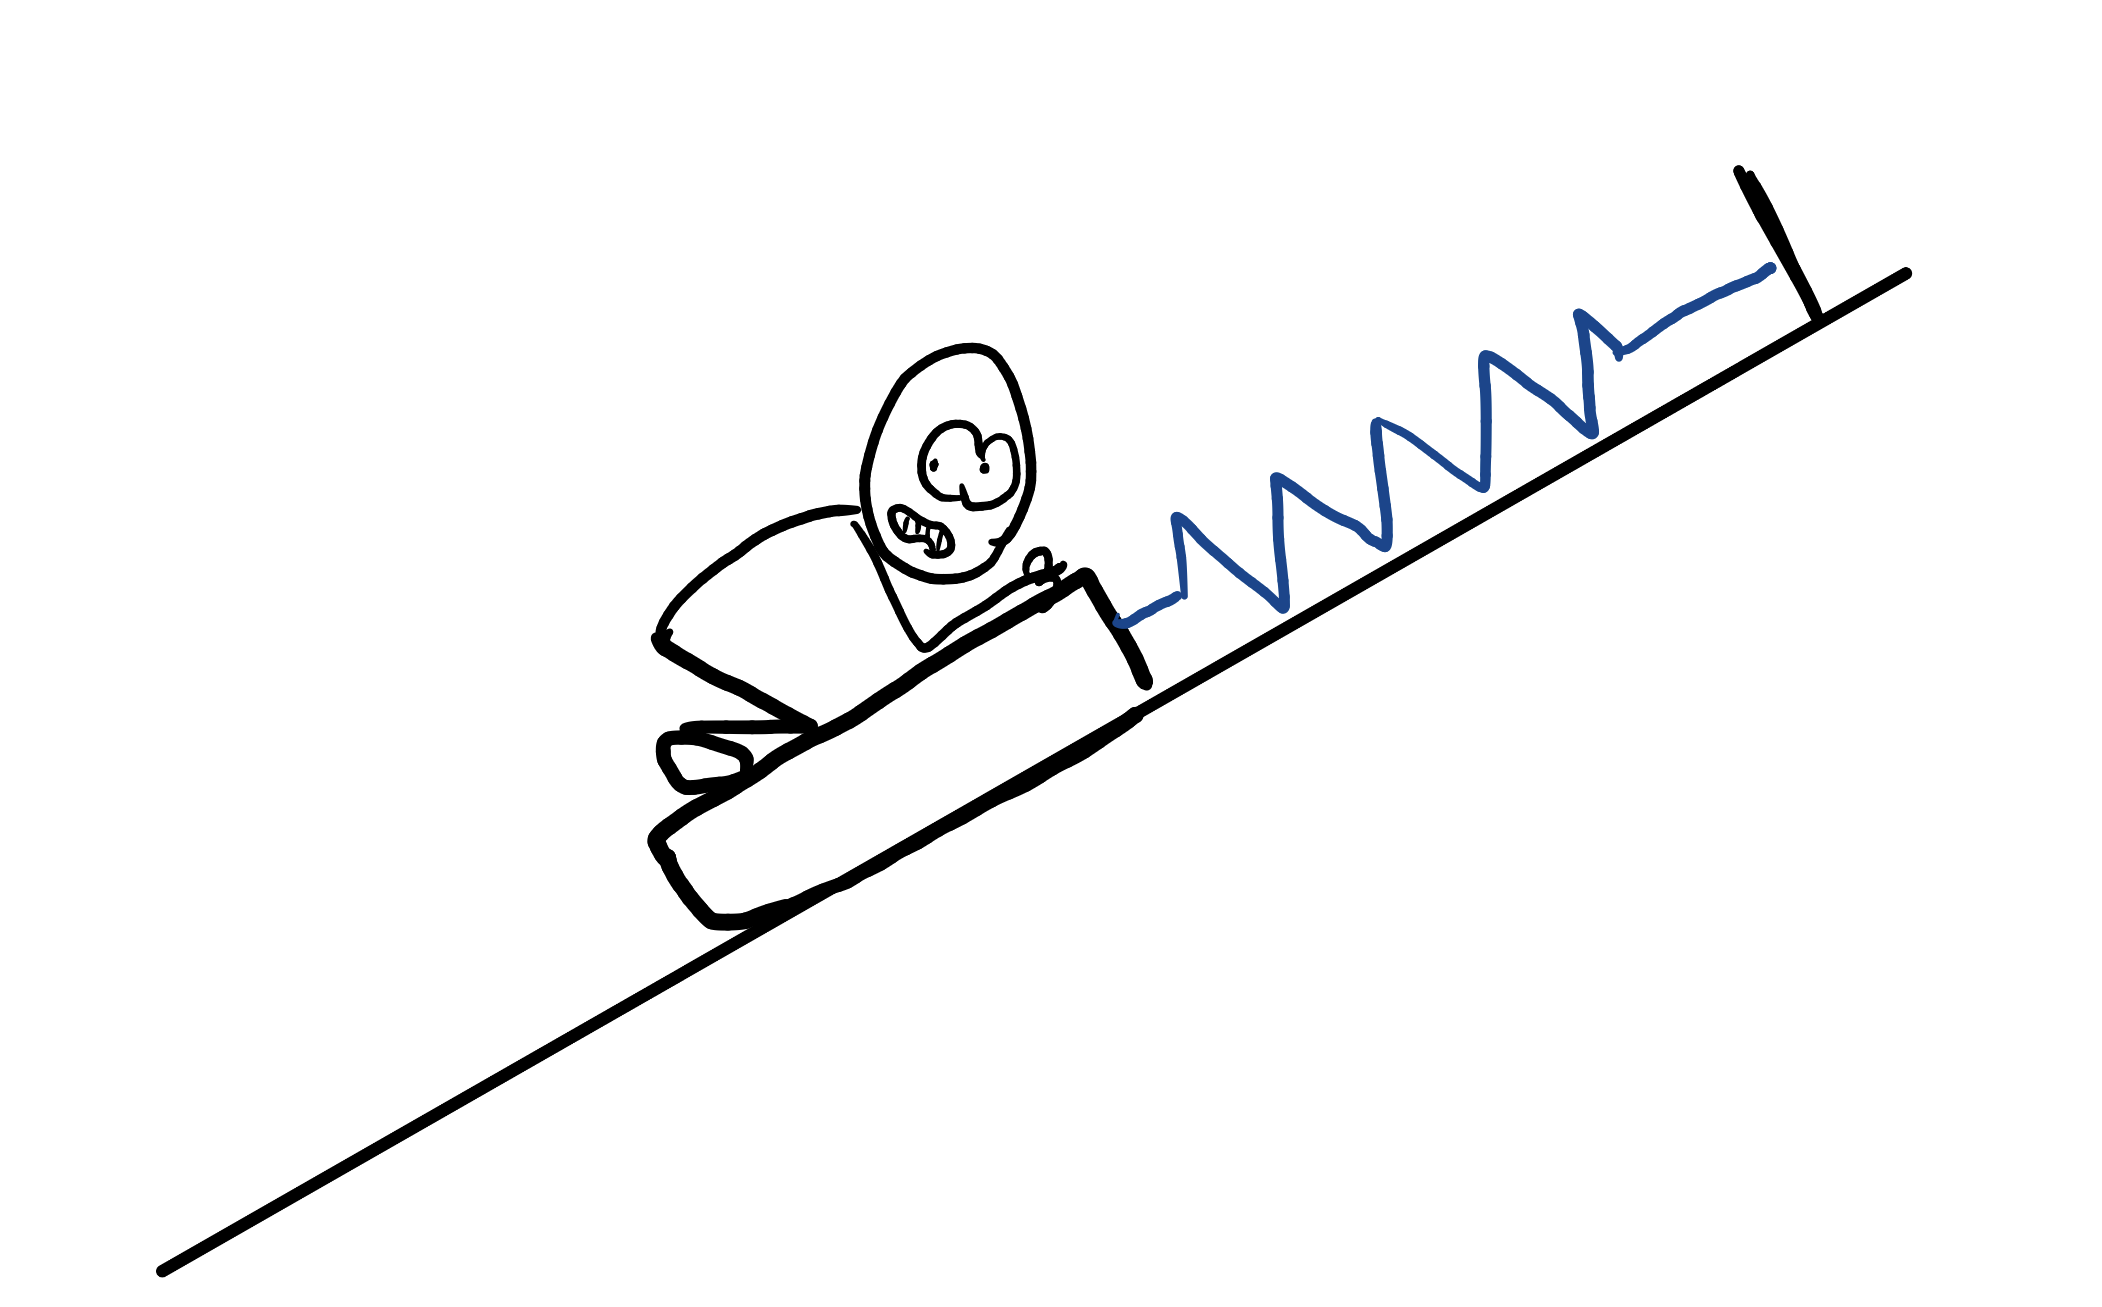
\includegraphics[width=0.86\textwidth]{Images/Kapittel4:Dynamikk/Dashman_slede_fjaer_skraplan.png}%
  };
\end{tikzpicture}
\caption{En slede (med Dashman) holdes i ro på et friksjonsfritt skråplan ($\theta=30°$) av en fjær festet til en stolpe på toppen av planet.}
\label{fig:slede_fjaer_skraplan}
\end{figure}

\exm{Slede i skråplan holdt av fjær}{%
En slede med Dashman, med samlet masse $m$, ligger i ro på et friksjonsfritt skråplan med helningsvinkel $\theta = 30°$ (se figur~\ref{fig:slede_fjaer_skraplan}). Sleden er festet til en fjær med fjærkonstant $k = \SI{180}{\newton\per\metre}$, som er strukket en lengde $x = \SI{12}{\centi\metre}$ fra likevekt.
\begin{enumerate}[a)]
    \item Tegn inn kreftene som virker på sleden.
    \item Regn ut fjærkrafta $F_k$.
    \item Finn massen $m$ til sleden (med Dashman).
\end{enumerate}
}

\svar{%
\noindent
\textbf{a) Figur og krefter:} Tre krefter virker på sleden: normalkraften $\vec{N}$ (vinkelrett på skråplanet), tyngdekraften $\vec{G}=m\vec{\mathrm{g}}$ (rett ned) og fjærkrafta $\vec{F}_k$ (langs skråplanet, oppover). Se figur~\ref{fig:slede_fjaer_skraplan_losning}.

\begin{center}
\begin{tikzpicture}
  \node[anchor=south west, inner sep=0] (image) at (0,0) {%
    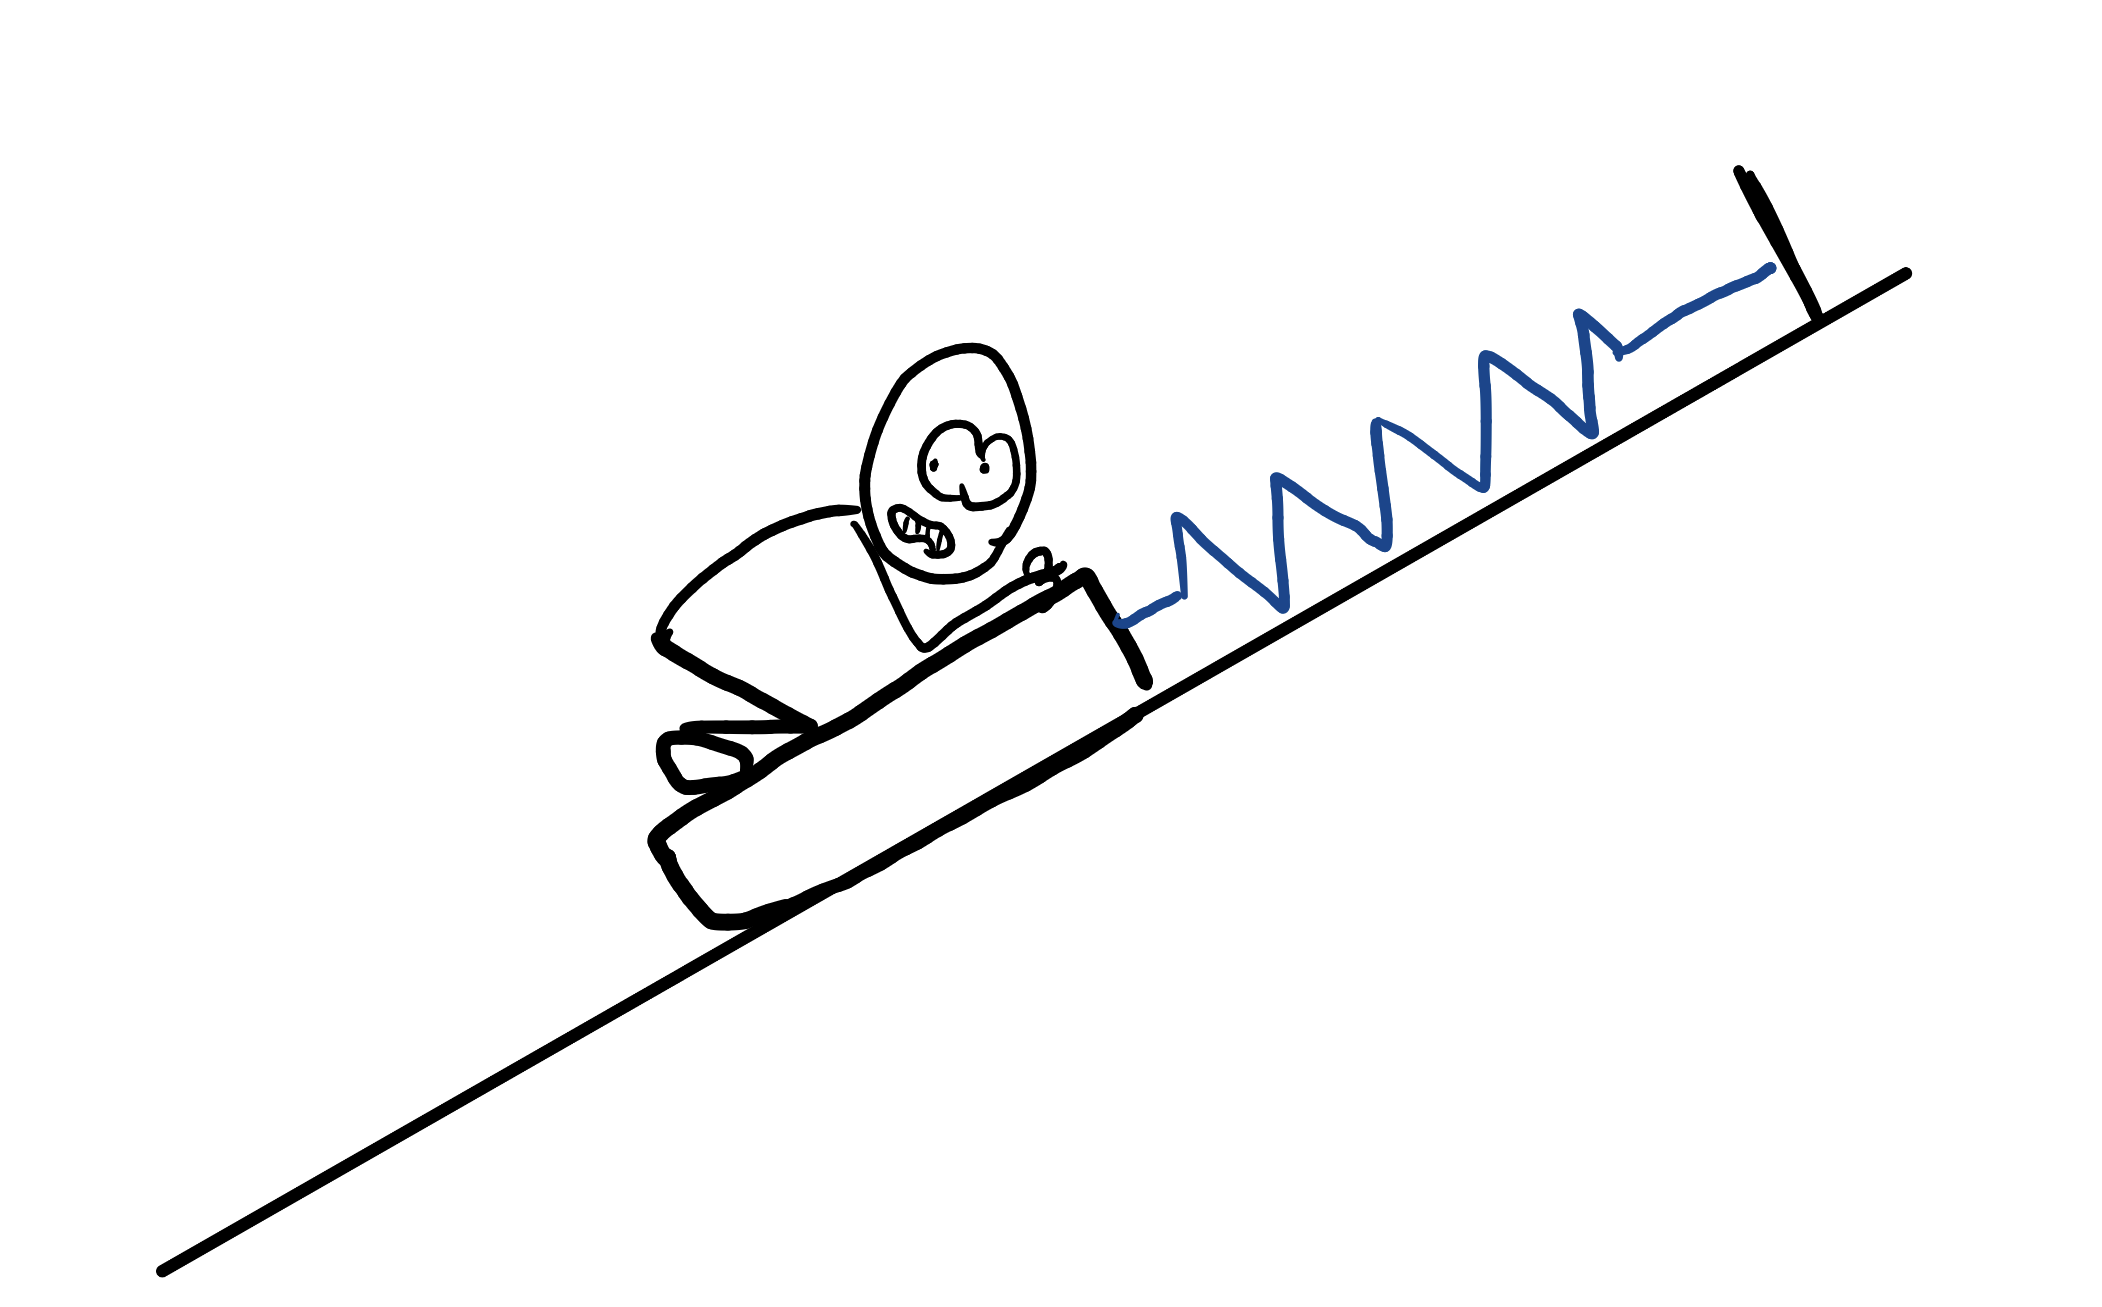
\includegraphics[width=0.72\textwidth]{Images/Kapittel4:Dynamikk/Dashman_slede_fjaer_skraplan.png}%
  };
  \begin{scope}[x={(image.south east)}, y={(image.north west)}]
    % N: normalkraft, vinkelrett på skråplanet
    \draw[-{Stealth[length=11pt,width=7pt]}, line width=2.5pt, defscol]
      (0.419,0.357) -- (0.3481,0.5562);
    \node[left=4pt, defscol, font=\small\bfseries,
          fill=white, draw=defscol, line width=0.3pt,
          inner sep=2pt, rounded corners=1pt]
      at (0.3481,0.5562) {$\vec{N}$};
    % G: tyngdekraft, rett ned
    \draw[-{Stealth[length=11pt,width=7pt]}, line width=2.5pt, black!65]
      (0.452,0.426) -- (0.452,0.1964);
    \node[below=4pt, black!65, font=\small\bfseries,
          fill=white, draw=black!50, line width=0.3pt,
          inner sep=2pt, rounded corners=1pt]
      at (0.452,0.1964) {$\vec{G}$};
    % Fk: fjærkraft, langs skråplanet oppover
    \draw[-{Stealth[length=11pt,width=7pt]}, line width=2.5pt, oppsumcol]
      (0.530,0.525) -- (0.6539,0.6391);
    \node[above=4pt, oppsumcol, font=\small\bfseries,
          fill=white, draw=oppsumcol, line width=0.3pt,
          inner sep=2pt, rounded corners=1pt]
      at (0.6539,0.6391) {$\vec{F}_k$};
    \fill[defscol] (0.419,0.357) circle (2pt);
    \fill[black!55] (0.452,0.426) circle (2pt);
    \fill[oppsumcol] (0.530,0.525) circle (2pt);
  \end{scope}
\end{tikzpicture}
\end{center}
\captionof{figure}{Krefter på sleden: normalkraft $\vec{N}$, tyngdekraft $\vec{G}$ og fjærkraft $\vec{F}_k$.}
\label{fig:slede_fjaer_skraplan_losning}

\smallskip\noindent
\textbf{Lov og koordinatsystem:} Sleden er i ro, så Newtons 1. lov gir $\sum\vec{F}=0$. Vi velger $x$-akse langs skråplanet (positiv oppover) og $y$-akse vinkelrett på skråplanet.

\smallskip\noindent
\textbf{Dekomponér langs skråplanet ($x$-retning):}
\[
    \sum F_x = F_k - m\mathrm{g}\sin\theta = 0
\]

\smallskip\noindent
\textbf{b) Fjærkrafta:}
\[
    F_k = kx = \SI{180}{\newton\per\metre}\cdot\SI{0.12}{\metre} = \doubleunderline{\SI{21.6}{\newton}}
\]

\smallskip\noindent
\textbf{c) Massen:} Fra dekomponeringen over har vi $F_k = m\mathrm{g}\sin\theta$, slik at
\[
    m = \frac{F_k}{\mathrm{g}\sin\theta}
    = \frac{\SI{21.6}{\newton}}{\SI{9.81}{\metre\per\second\squared}\cdot\sin 30°}
    = \doubleunderline{\SI{4.4}{\kilo\gram}}
\]
}

\noindent
\begin{minipage}[t]{0.52\linewidth}
\vspace{0pt}
\oppgaver{Kjelke med skrå trekkraft}{k4oppg9}{%
%
En kjelke med masse $m = \SI{15}{\kilo\gram}$ dras langs et flatt, snødekket underlag. Trekkraften $\vec{F} = \SI{50}{\newton}$ er rettet i vinkel $\theta = 30°$ over horisontal (se figur). Den kinetiske friksjonskoeffisienten er $\mu_k = 0.20$.
\begin{enumerate}[a)]
    \item Finn normalkraften $N$. (Husk at $\vec{F}$ har en vertikal komponent som påvirker $N$.)
    \item Finn friksjonskraften $R$.
    \item Finn kjelkens akselerasjon.
\end{enumerate}
%
}
\end{minipage}%
\hfill
\begin{minipage}[t]{0.45\linewidth}
\vspace{6pt}
\centering
\begin{tikzpicture}[font=\small]
  % Surface
  \fill[black!12] (-0.7,-0.38) rectangle (4.7,0);
  \draw[very thick] (-0.7,0) -- (4.7,0);
  \foreach \x in {-0.55,-0.30,...,4.55} {
    \draw[black!35, thin] (\x,0) -- (\x-0.22,-0.22);
  }
  % Kjelke (lavere profil)
  \fill[headCol!20] (0.80,0) rectangle (2.80,0.90);
  \draw[headCol!65!black, thick] (0.80,0) rectangle (2.80,0.90);
  \node at (2.15,0.45) {$m$};
  % N: normalkraft opp fra kontaktflate
  \draw[-{Stealth[length=11pt,width=7pt]}, line width=2.5pt, defscol]
    (1.50, 0) -- (1.50, 1.60);
  \node[left=5pt, defscol, font=\small\bfseries,
        fill=white, draw=defscol, line width=0.3pt,
        inner sep=2pt, rounded corners=1pt]
    at (1.50, 1.28) {$\vec{N}$};
  % G: tyngdekraft ned fra massesentrum
  \draw[-{Stealth[length=11pt,width=7pt]}, line width=2.5pt, black!65]
    (1.80, 0.45) -- (1.80, -0.70);
  \node[right=5pt, black!65, font=\small\bfseries,
        fill=white, draw=black!50, line width=0.3pt,
        inner sep=2pt, rounded corners=1pt]
    at (1.80, -0.07) {$\vec{G}$};
  % F: trekkraft i 30 grader (cos30=0.866, sin30=0.5; L=1.12)
  \draw[-{Stealth[length=11pt,width=7pt]}, line width=2.5pt, oppsumcol]
    (2.80, 0.45) -- (3.77, 1.01);
  \node[right=4pt, oppsumcol, font=\small\bfseries] at (3.77, 1.01) {$\vec{F}$};
  % Stiplet horisontal referanselinje for vinkel
  \draw[black!35, thin, dashed] (2.80,0.45) -- (3.55,0.45);
  % Vinkelbue 0 -> 30 grader, radius 0.48, sentrum (2.80,0.45)
  \draw[black!60, thin] (3.28,0.45) arc (0:30:0.48);
  \node[black!70, font=\scriptsize] at (3.43, 0.58) {$\theta$};
  % R: friksjonskraft venstre fra kontaktflate (lenger bak på klossen, forbi N)
  \draw[-{Stealth[length=11pt,width=7pt]}, line width=2.5pt, red!70!black]
    (1.20, 0) -- (-0.20, 0);
  \node[below=5pt, red!70!black, font=\small\bfseries,
        fill=white, draw=red!70!black, line width=0.3pt,
        inner sep=2pt, rounded corners=1pt]
    at (0.50, 0) {$\vec{R}$};
  % Prikker ved angrepspunkt
  \fill[defscol] (1.50, 0) circle (2pt);
  \fill[red!70!black] (1.20, 0) circle (2pt);
  \fill[black!55] (1.80, 0.45) circle (2pt);
\end{tikzpicture}
\captionof{figure}{Kjelke dradd med kraft $\vec{F}$ i vinkel $\theta=30°$ over horisontal. Friksjonskraften $\vec{R}$ og normalkraften $\vec{N}$ angriper ved kontaktflaten.}
\label{fig:kjelke}
\end{minipage}

\subsection{Skråplan}
\begin{wrapfigure}[6]{r}[1.5cm]{3.6cm}
\vspace{-\baselineskip}%
\rotatebox{-15}{\href{https://youtu.be/yUWWR755VEY?si=j16Huykhv5B3eNVR}{%
\begin{tikzpicture}[inner sep=0pt]
\node[anchor=south west] (thumb) at (0,0) {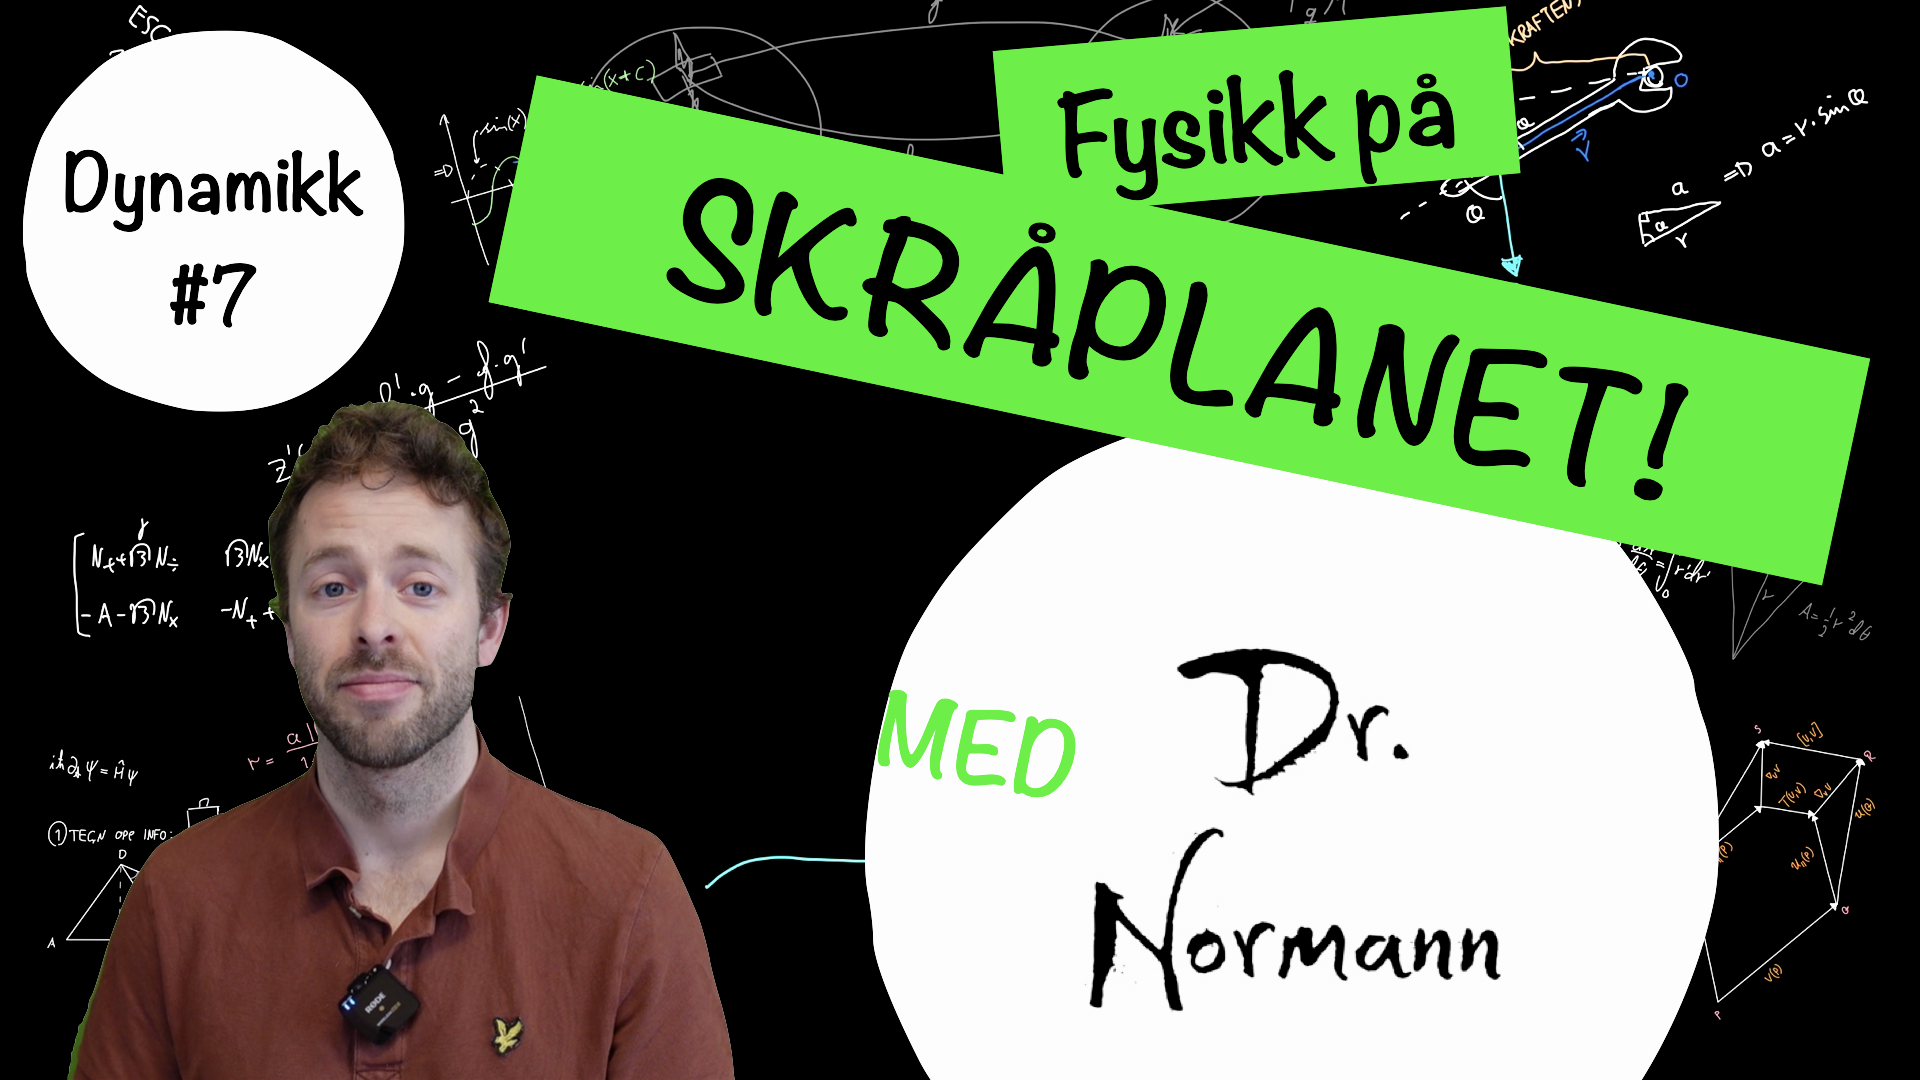
\includegraphics[width=3.6cm]{Images/YouTubeLenker/YT_Skraplanet.png}};
\node[anchor=north west] at (thumb.south west) {
\includegraphics[width=1.2cm]{Images/YouTubeLenker/Icon.png}};
\end{tikzpicture}%
}}%
\end{wrapfigure}
Et legeme på skråplan er et mye brukt eksempel som gir oss anledning til å øve på å anvende tre av kreftene vi har pratet om så langt ($\vec{G}, \vec{N}$ og $\vec{R}$) samtidig. I tillegg gir det god øvelse i dekomponering, som vi skal se. La oss se for oss en bil i en isete bakke. Vi ønsker å kunne besvare spørsmål som
\begin{itemize}
    \item Ved hvilken vinkel begynner bilen å skli?
    \item Hvor fort akselererer den nedover bakken når den først sklir?
\end{itemize}
La oss nå besvare disse to spørsmålene systematisk ved å bruke Newtons 2. lov. Figur~\ref{fig:skråplankrefter1} viser kreftene som virker på en kloss som sklir nedover et skråplan med helningsvinkel $\theta$.

\begin{figure}[ht!]
    \centering
    \begin{tikzpicture}[font=\small]
      % Bakke (horisontal)
      \draw[thick] (-4.3,0) -- (0.3,0);
      % Skråplan (opp mot venstre, theta=25 grader — visuelt representativt)
      \draw[very thick] (0,0) -- (-3.81,1.77);
      % Vinkelbue theta ved basen
      \draw[black!55,thin] (-0.55,0) arc (180:155:0.55);
      \node[font=\scriptsize,black!70] at (-0.62,0.16) {$\theta$};

      % Kloss (tiltet)
      \fill[headCol!20] (-2.538,1.183) -- (-1.722,0.803) -- (-1.502,1.274) -- (-2.318,1.655) -- cycle;
      \draw[headCol!65!black,thick] (-2.538,1.183) -- (-1.722,0.803) -- (-1.502,1.274) -- (-2.318,1.655) -- cycle;
      \node[font=\scriptsize] at (-2.02,1.23) {$m$};

      % N (grønn), normalt ut fra planet
      \draw[-{Stealth[length=10pt,width=6pt]}, line width=2.2pt, defscol]
        (-2.130,0.993) -- (-1.475,2.398);
      \node[above=1pt,defscol,font=\small\bfseries,fill=white,draw=defscol,
            line width=0.3pt,inner sep=2pt,rounded corners=1pt] at (-1.475,2.398) {$\vec{N}$};

      % R (rød), friksjon opp langs planet (motsatt av bevegelsesretningen)
      \draw[-{Stealth[length=10pt,width=6pt]}, line width=2.2pt, red!70!black]
        (-2.538,1.183) -- (-3.489,1.627);
      \node[above=1pt,red!70!black,font=\small\bfseries,fill=white,draw=red!70!black,
            line width=0.3pt,inner sep=2pt,rounded corners=1pt] at (-3.489,1.627) {$\vec{R}$};

      % Fartsretning, adskilt fra klossen
      \draw[-{Stealth[length=8pt,width=5pt]}, line width=1.3pt, violet!55]
        (-1.450,0.676) -- (-0.680,0.317);

      % G (blå), rett ned fra massesenteret
      \draw[-{Stealth[length=10pt,width=6pt]}, line width=2.2pt, blue!55!black]
        (-2.020,1.229) -- (-2.020,-0.521);
      \node[left=1pt,blue!55!black,font=\small\bfseries,fill=white,draw=blue!55!black,
            line width=0.3pt,inner sep=2pt,rounded corners=1pt] at (-2.020,-0.30) {$\vec{G}$};

      % Gx, Gy: komponenter av G, stiplet
      \draw[-{Stealth[length=7pt,width=4pt]}, line width=1.2pt, dashed, cyan!70!blue]
        (-2.020,1.229) -- (-1.350,0.916);
      \node[above=1pt,cyan!70!blue,font=\scriptsize] at (-1.30,0.99) {$G_x$};
      \draw[-{Stealth[length=7pt,width=4pt]}, line width=1.2pt, dashed, cyan!70!blue]
        (-2.020,1.229) -- (-2.690,-0.209);
      \node[left=1pt,cyan!70!blue,font=\scriptsize] at (-2.690,-0.209) {$G_y$};

      % Vinkelbue theta mellom G og Gy
      \draw[black!50,thin] (-2.020,0.879) arc (245:270:0.35);
      \node[black!65,font=\scriptsize] at (-2.13,0.75) {$\theta$};

      % Prikker ved kraftangrepspunkt
      \fill[black!60] (-2.130,0.993) circle (1.5pt);
      \fill[black!60] (-2.020,1.229) circle (1.5pt);

      % Koordinatsystem (x nedover skråplanet, y normalt ut)
      \draw[-{Stealth[length=7pt,width=5pt]},black!70,semithick]
        (1.05,1.55) -- (1.639,1.275);
      \node[right=1pt,black!70,font=\scriptsize] at (1.639,1.275) {$x$};
      \draw[-{Stealth[length=7pt,width=5pt]},black!70,semithick]
        (1.05,1.55) -- (1.325,2.139);
      \node[above=1pt,black!70,font=\scriptsize] at (1.325,2.139) {$y$};
      \fill[black!70] (1.05,1.55) circle (1pt);
    \end{tikzpicture}
    \caption{Krefter på en kloss som sklir nedover et skråplan. Normalkraften $\vec{N}$ peker normalt ut fra planet, tyngdekraften $\vec{G}$ peker rett ned (med komponenter $G_x$, $G_y$ langs og normalt på planet), og friksjonskraften $\vec{R}$ peker opp langs planet siden klossen beveger seg ned. Koordinatsystem: $x$ nedover langs planet, $y$ normalt ut.}
    \label{fig:skråplankrefter1}
\end{figure}

\paragraph*{Utledning av akselerasjon ned et skråplan med friksjon.}

\noindent
\textbf{1. Figur:} Se figur~\ref{fig:skråplankrefter1}.

\smallskip\noindent
\textbf{2. Lov:} Klossen akselererer nedover langs planet med $\vec{a}$ ned bakken. Friksjonskraften er glidefriksjon og peker \textit{opp} langs planet (den motvirker bevegelsen): $R = \mu_k N$.

\smallskip\noindent
\textbf{3. Koordinatsystem:} Vi velger $x$ nedover langs planet (positiv retning ned bakken) og $y$ normalt ut fra overflaten. Klossen beveger seg bare langs $x$, så $a_y = 0$.

\smallskip\noindent
\textbf{4. Dekomponér:}
\begin{align*}
    \sum F_y = 0 &:\quad N - m\mathrm{g}\cos\theta = 0 \implies N = m\mathrm{g}\cos\theta\\
    \sum F_x = ma &:\quad m\mathrm{g}\sin\theta - R = ma
\end{align*}

\smallskip\noindent
\textbf{5. Løs:} Setter inn $R = \mu_k N = \mu_k m\mathrm{g}\cos\theta$:
\begin{align*}
    m\mathrm{g}\sin\theta - \mu_k m\mathrm{g}\cos\theta &= ma\\
    \mathrm{g}(\sin\theta - \mu_k\cos\theta) &= a
\end{align*}

\begin{tcolorbox}[colback=gray!13, colframe=gray!40, boxrule=0.5pt, top=5pt, bottom=5pt, left=8pt, right=8pt]
\[
    a = \mathrm{g}(\sin\theta - \mu_k\cos\theta)
\]
\end{tcolorbox}

\noindent
Legg merke til at massen $m$ falt ut av ligningen. Akselerasjonen ned et skråplan er uavhengig av massen — en tung buss og en lett sykkel akselererer like fort nedover den samme bakken.

\medskip

\paragraph*{Kritisk vinkel — ved hvilken helning begynner klossen å skli?}

Klossen er nettopp på grensen til å begynne å skli når tyngdekraftens komponent langs planet er lik den maksimale hvilefriksjonen. I dette grensetilfelle er $\sum F_x = 0$ med $R_s = \mu_s N$ (maksimal hvilefriksjon):
\[
m\mathrm{g}\sin\theta_c - \mu_s m\mathrm{g}\cos\theta_c = 0
\quad\implies\quad
\tan\theta_c = \mu_s
\]

\begin{tcolorbox}[colback=gray!13, colframe=gray!40, boxrule=0.5pt, top=5pt, bottom=5pt, left=8pt, right=8pt]
\[
    \theta_c = \arctan(\mu_s)
\]
\end{tcolorbox}

\noindent
Er $\theta < \theta_c$ holder friksjonskraften klossen i ro. Er $\theta > \theta_c$ begynner klossen å skli.

\oppgaver{Buss på glatt vei}{k4oppg10}{%
%
En buss parkerer på en bakke. Friksjonskoeffisientene mellom dekk og vei er $\mu_s = 0.70$ (statisk) og $\mu_k = 0.50$ (kinetisk).
\begin{enumerate}[a)]
    \item Ved hvilken helningsvinkel $\theta_c$ begynner bussen å skli nedover?
    \item Hva blir akselerasjonen til bussen idet den begynner å skli?
\end{enumerate}
%
}

\medskip

% ---- Eksempel 2: Kloss på skråplan holdt av fjær og friksjon ----
\noindent
\begin{minipage}[t]{0.54\linewidth}
\vspace{0pt}
I neste eksempel kombinerer vi fjærkraft og friksjon på et skråplan. Koordinatsystemet velges med $x$-aksen langs planet (positiv retning opp bakken) og $y$-aksen normalt ut fra overflaten. Figuren viser en kloss som er på grensen til å gli nedover, slik at $R = \mu_s N$ (maks hvilefriksjon).
\end{minipage}%
\hfill
\begin{minipage}[t]{0.43\linewidth}
\vspace{0pt}
\centering
\begin{tikzpicture}[font=\small]
  % Skråplan-kropp (theta=30 grader, forstørret med faktor 1.3: 3.46*1.3=4.498, 2.0*1.3=2.6)
  \fill[black!12] (0,0) -- (4.498,2.6) -- (4.498,0) -- cycle;
  \draw[very thick] (0,0) -- (4.498,2.6);
  \draw[very thick] (0,0) -- (4.498,0);
  \draw[thick,black!50] (4.498,0) -- (4.498,2.6);
  % Vinkelmerke
  \draw[black!55,thin] (0.845,0) arc (0:30:0.845);
  \node[font=\scriptsize,black!70] at (1.066,0.208) {$\theta$};
  % Vegg venstre
  \fill[black!15] (-0.455,0) rectangle (0,0.715);
  \draw[very thick] (0,0) -- (0,0.715);
  \foreach \y in {0.065,0.26,0.455,0.65} {
    \draw[black!40,thin] (0,\y) -- (-0.325,\y+0.26);
  }
  % Fjær langs planet (rotert 30 grader), hevet til klossens midthøyde (lokal y=0.312)
  % slik at den møter klossen midt på sideflaten, ikke i et hjørne
  \begin{scope}[rotate=30, yshift=0.312cm]
    \draw[line width=1.2pt,headCol!70!black]
      (0.104,0) -- (0.286,0)
      -- (0.442,0.221) -- (0.598,-0.221) -- (0.754,0.221)
      -- (0.910,-0.221) -- (1.066,0.221) -- (1.222,-0.221)
      -- (1.378,0.221) -- (1.534,0) -- (1.690,0);
  \end{scope}
  % Kloss (rotert 30 grader), hevet slik at underkanten ligger på planet
  % (lokal y: 0 til 0.624 -- klossen står PÅ planet, ikke halvveis nedi det)
  % Klosssenter i rotert ramme: (2.21, 0.312)
  \begin{scope}[rotate=30]
    \fill[headCol!20] (1.755,0) rectangle (2.665,0.624);
    \draw[headCol!65!black,thick] (1.755,0) rectangle (2.665,0.624);
    \node[font=\scriptsize] at (2.21,0.16) {$m$};
  \end{scope}
  % Koordinataksene (langs planet), tegnet som eget lite koordinatsystem
  % i ledig plass oppe til venstre -- uavhengig av kraftvektorene, slik at
  % y-aksen (normalt ut) ikke smelter sammen med normalkraften $\vec{N}$
  \draw[-{Stealth[length=7pt,width=5pt]},black!70,semithick]
    (0.30,1.35) -- (0.90,1.65);
  \node[right=2pt,black!70,font=\scriptsize] at (0.90,1.65) {$x$};
  \draw[-{Stealth[length=7pt,width=5pt]},black!70,semithick]
    (0.30,1.35) -- (0.00,1.92);
  \node[above=1pt,black!70,font=\scriptsize] at (0.00,1.92) {$y$};
  \fill[black!70] (0.30,1.35) circle (1.5pt);
  % N: normalt ut fra bunnflate (1.914, 1.105)
  % Retning: (-0.5, 0.866), lengde 1.17. Tupp: (1.329, 2.118)
  \draw[-{Stealth[length=11pt,width=7pt]}, line width=2.5pt, defscol]
    (1.914,1.105) -- (1.329,2.118);
  \node[above left=2pt,defscol,font=\small\bfseries,fill=white,draw=defscol,
        line width=0.3pt,inner sep=2pt,rounded corners=1pt]
    at (1.329,2.118) {$\vec{N}$};
  % G: ned fra massesentrum (1.758, 1.375)
  \draw[-{Stealth[length=11pt,width=7pt]}, line width=2.5pt, black!65]
    (1.758,1.375) -- (1.758,-0.26);
  \node[right=4pt,black!65,font=\small\bfseries,fill=white,draw=black!50,
        line width=0.3pt,inner sep=2pt,rounded corners=1pt]
    at (1.758,0.30) {$\vec{G}$};
  % F_fjær: opp langs planet fra venstre flate, i klossens midthøyde (1.364, 1.148)
  % Retning: (0.866,0.5), lengde 1.04. Tupp: (2.265, 1.668)
  \draw[-{Stealth[length=11pt,width=7pt]}, line width=2.5pt, oppsumcol]
    (1.364,1.148) -- (2.265,1.668);
  \node[above=6pt,oppsumcol,font=\small\bfseries,fill=white,draw=oppsumcol,
        line width=0.3pt,inner sep=2pt,rounded corners=1pt]
    at (2.265,1.668) {$\vec{F}$};
  % R: opp langs planet fra bunnflate (1.914, 1.105)
  % Retning: (0.866,0.5), lengde 0.91. Tupp: (2.702, 1.560)
  \draw[-{Stealth[length=11pt,width=7pt]}, line width=2.5pt, red!70!black]
    (1.914,1.105) -- (2.702,1.560);
  \node[below right=2pt,red!70!black,font=\small\bfseries,fill=white,draw=red!70!black,
        line width=0.3pt,inner sep=2pt,rounded corners=1pt]
    at (2.702,1.560) {$\vec{R}$};
  % Prikker
  \fill[defscol] (1.914,1.105) circle (2pt);
  \fill[red!70!black] (1.914,1.105) circle (2pt);
  \fill[black!55] (1.758,1.375) circle (2pt);
\end{tikzpicture}
\captionof{figure}{Kloss på skråplan ($\theta=30°$) holdt av fjær $\vec{F}$ og friksjon $\vec{R}$. Koordinatsystem: $x$ opp langs planet, $y$ normalt ut.}
\label{fig:kloss_fjaer_skraa}
\end{minipage}

\medskip

\exm{Kloss på skråplan — fjær og friksjon}{%
En kloss med masse $m = \SI{2.0}{\kilo\gram}$ ligger på et skråplan med helningsvinkel $\theta = 30°$. En fjær langs planet er festet mellom klossen og en vegg i bunnen av bakken, og er komprimert $x = \SI{3.0}{\centi\metre}$. Klossen er akkurat på grensen til å gli nedover, og den statiske friksjonskoeffisienten er $\mu_s = 0.20$. Finn fjærkonstanten $k$.
}

\svar{%
\noindent
\textbf{1. Figur:} Se figur over.

\smallskip\noindent
\textbf{2. Lov:} Klossen er (nesten) i ro: $\sum\vec{F}=0$. Maks hvilefriksjon gjelder: $R = \mu_s N$.

\smallskip\noindent
\textbf{3. Koordinatsystem:} $x$ opp langs planet, $y$ normalt ut fra planet.

\smallskip\noindent
\textbf{4. Dekomponér:}
\begin{align*}
    \sum F_y = 0&:\quad N - G\cos\theta = 0 \implies N = m\mathrm{g}\cos\theta\\
    \sum F_x = 0&:\quad kx + R - G\sin\theta = 0
\end{align*}

\smallskip\noindent
\textbf{5. Løs:} Sett inn $R = \mu_s N = \mu_s m\mathrm{g}\cos\theta$:
\[
    kx = m\mathrm{g}\sin\theta - \mu_s m\mathrm{g}\cos\theta = m\mathrm{g}(\sin\theta - \mu_s\cos\theta)
\]
\[
    k = \frac{m\mathrm{g}(\sin\theta - \mu_s\cos\theta)}{x}
    = \frac{\SI{2.0}{\kilo\gram}\cdot\SI{9.81}{\metre\per\second\squared}(\sin 30° - 0.20\cdot\cos 30°)}{\SI{0.030}{\metre}}
    = \doubleunderline{\SI{214}{\newton\per\metre}}
\]
}



\exm{Kloss på skråplan}{%
En kloss med masse $m = \SI{3.0}{\kilo\gram}$ beveger seg nedover et skråplan med helningsvinkel $\theta = 25°$, med akselerasjon $a = \SI{3.0}{\metre\per\second\squared}$ (se figur~\ref{fig:skråplankrefter}).
\begin{enumerate}[a)]
    \item Finn friksjonskrafta $R$ som virker på klossen.
    \item Finn normalkraften $N$.
\end{enumerate}
}

\svar{%
\noindent
\textbf{1. Figur:} Se figur~\ref{fig:skråplankrefter}. Kreftene som virker på klossen er tyngdekraften $\vec{G}$, normalkraften $\vec{N}$ og friksjonskraften $\vec{R}$.

\smallskip\noindent
\textbf{2. Lov:} Klossen akselererer langs planet, så Newtons 2. lov gir $\sum\vec{F}=m\vec{a}$.

\smallskip\noindent
\textbf{3. Koordinatsystem:} $x$-akse langs skråplanet (positiv nedover, i bevegelsesretningen), $y$-akse normalt på skråplanet.

\smallskip\noindent
\textbf{4. Dekomponér:}
\begin{align*}
    \sum F_x = ma&:\quad G\sin\theta - R = ma\\
    \sum F_y = 0&:\quad N - G\cos\theta = 0
\end{align*}

\smallskip\noindent
\textbf{5. Løs:}

\noindent
\textbf{a)} Fra $x$-likningen:
\[
    R = G\sin\theta - ma = m(\mathrm{g}\sin\theta - a)
    = \SI{3.0}{\kilo\gram}\left(\SI{9.81}{\metre\per\second\squared}\cdot\sin 25° - \SI{3.0}{\metre\per\second\squared}\right)
    = \doubleunderline{\SI{3.4}{\newton}}
\]
Positivt fortegn betyr at friksjonen peker oppover langs planet (motsatt av bevegelsesretningen), som forventet.

\smallskip\noindent
\textbf{b)} Fra $y$-likningen:
\[
    N = G\cos\theta = m\mathrm{g}\cos\theta
    = \SI{3.0}{\kilo\gram}\cdot\SI{9.81}{\metre\per\second\squared}\cdot\cos 25°
    = \doubleunderline{\SI{26.7}{\newton}}
\]
}


\begin{figure}[ht!]
    \centering
    \begin{tikzpicture}[font=\small]
      % Bakke (horisontal)
      \draw[thick] (-4.3,0) -- (0.3,0);
      % Skråplan (opp mot venstre, theta=25 grader — visuelt representativt)
      \draw[very thick] (0,0) -- (-3.81,1.77);
      % Vinkelbue theta ved basen
      \draw[black!55,thin] (-0.55,0) arc (180:155:0.55);
      \node[font=\scriptsize,black!70] at (-0.62,0.16) {$\theta$};

      % Kloss (tiltet)
      \fill[headCol!20] (-2.538,1.183) -- (-1.722,0.803) -- (-1.502,1.274) -- (-2.318,1.655) -- cycle;
      \draw[headCol!65!black,thick] (-2.538,1.183) -- (-1.722,0.803) -- (-1.502,1.274) -- (-2.318,1.655) -- cycle;
      \node[font=\scriptsize] at (-2.02,1.23) {$m$};

      % N (grønn), normalt ut fra planet
      \draw[-{Stealth[length=10pt,width=6pt]}, line width=2.2pt, defscol]
        (-2.130,0.993) -- (-1.475,2.398);
      \node[above=1pt,defscol,font=\small\bfseries,fill=white,draw=defscol,
            line width=0.3pt,inner sep=2pt,rounded corners=1pt] at (-1.475,2.398) {$\vec{N}$};

      % R (rød), friksjon opp langs planet (motsatt av bevegelsesretningen)
      \draw[-{Stealth[length=10pt,width=6pt]}, line width=2.2pt, red!70!black]
        (-2.538,1.183) -- (-3.489,1.627);
      \node[above=1pt,red!70!black,font=\small\bfseries,fill=white,draw=red!70!black,
            line width=0.3pt,inner sep=2pt,rounded corners=1pt] at (-3.489,1.627) {$\vec{R}$};

      % Fartsretning, adskilt fra klossen
      \draw[-{Stealth[length=8pt,width=5pt]}, line width=1.3pt, violet!55]
        (-1.450,0.676) -- (-0.680,0.317);

      % G (blå), rett ned fra massesenteret
      \draw[-{Stealth[length=10pt,width=6pt]}, line width=2.2pt, blue!55!black]
        (-2.020,1.229) -- (-2.020,-0.521);
      \node[left=1pt,blue!55!black,font=\small\bfseries,fill=white,draw=blue!55!black,
            line width=0.3pt,inner sep=2pt,rounded corners=1pt] at (-2.020,-0.30) {$\vec{G}$};

      % Gx, Gy: komponenter av G, stiplet
      \draw[-{Stealth[length=7pt,width=4pt]}, line width=1.2pt, dashed, cyan!70!blue]
        (-2.020,1.229) -- (-1.350,0.916);
      \node[above=1pt,cyan!70!blue,font=\scriptsize] at (-1.30,0.99) {$G_x$};
      \draw[-{Stealth[length=7pt,width=4pt]}, line width=1.2pt, dashed, cyan!70!blue]
        (-2.020,1.229) -- (-2.690,-0.209);
      \node[left=1pt,cyan!70!blue,font=\scriptsize] at (-2.690,-0.209) {$G_y$};

      % Vinkelbue theta mellom G og Gy
      \draw[black!50,thin] (-2.020,0.879) arc (245:270:0.35);
      \node[black!65,font=\scriptsize] at (-2.13,0.75) {$\theta$};

      % Prikker ved kraftangrepspunkt
      \fill[black!60] (-2.130,0.993) circle (1.5pt);
      \fill[black!60] (-2.020,1.229) circle (1.5pt);

      % Koordinatsystem (x nedover skråplanet, y normalt ut)
      \draw[-{Stealth[length=7pt,width=5pt]},black!70,semithick]
        (1.05,1.55) -- (1.639,1.275);
      \node[right=1pt,black!70,font=\scriptsize] at (1.639,1.275) {$x$};
      \draw[-{Stealth[length=7pt,width=5pt]},black!70,semithick]
        (1.05,1.55) -- (1.325,2.139);
      \node[above=1pt,black!70,font=\scriptsize] at (1.325,2.139) {$y$};
      \fill[black!70] (1.05,1.55) circle (1pt);
    \end{tikzpicture}
    \caption{Krefter på en kloss på et skråplan. Tyngdekraften $\vec{G}$ dekomponeres i $G_x$ (langs planet) og $G_y$ (normalt på planet). Koordinatsystem: $x$ nedover langs planet, $y$ normalt ut.}
    \label{fig:skråplankrefter}
    \end{figure}
\newpage

\subsection{Krefter i sirkelbevegelse}
For sirkelbevegelse med konstant fart har vi sett at akselerasjonens størrelse er gitt ved
\[a=\frac{v^2}{r},\]
hvor $r$ er sirkelens radius. Om vi nå samstiller dette med Newtons 2. lov, $\sum\vec{F}=m\vec{a}$ så finner vi et uttrykk for kraftsummen inn mot sentrum.

\defn{Sentripetalkraft}{
Kraftsummen for sirkelbevegelse med radius $r$ og konstant banefart $v$ er gitt ved
\[\sum F=m\cdot \frac{v^2}{r},\]
og rettet inn mot sentrum av sirkelbevegelsen.
}


% ---- Eksempel: Ball i sirkelbane ----
\noindent
\begin{minipage}[t]{0.54\linewidth}
\vspace{0pt}
Som et første eksempel ser vi på en ball som glir rundt i en sirkelbane på en friksjonsfri horisontal overflate, festet til et senter med en snor. Snorkraften $\vec{S}$ peker hele tiden inn mot sentrum — det er denne kraften som gir ballen sentripetalakselerasjonen.
\end{minipage}%
\hfill
\begin{minipage}[t]{0.43\linewidth}
\vspace{0pt}
\centering
\begin{tikzpicture}[font=\small]
  % Sirkelbane (stiplet)
  \draw[dashed, gray!60, line width=0.8pt] (0,0) circle (1.5);
  % Sentrum
  \fill[black!60] (0,0) circle (2pt);
  \node[font=\scriptsize, below left=2pt] at (0,0) {sentrum};
  % Snor
  \draw[headCol!70!black, line width=1.4pt] (0,0) -- (1.5,0);
  % Ball
  \fill[headCol!40] (1.5,0) circle (0.18);
  \draw[headCol!70!black, line width=1pt] (1.5,0) circle (0.18);
  \node[font=\scriptsize, right=3pt] at (1.68,0) {$m$};
  % Snorkraft S (innover)
  \draw[-{Stealth[length=10pt,width=6pt]}, line width=2pt, defscol]
    (1.32,0) -- (0.35,0);
  \node[defscol, font=\small\bfseries, below=3pt] at (0.84,0) {$\vec{S}$};
  % Hastighet v (tangent, oppover)
  \draw[-{Stealth[length=10pt,width=6pt]}, line width=2pt, oppsumcol]
    (1.5,0.18) -- (1.5,1.10);
  \node[oppsumcol, font=\small\bfseries, right=3pt] at (1.5,0.64) {$\vec{v}$};
  % Radius r
  \draw[<->, gray!70, thin] (0,-0.35) -- (1.5,-0.35);
  \node[font=\scriptsize, gray!70, below] at (0.75,-0.35) {$r$};
\end{tikzpicture}
\captionof{figure}{Sett ovenfra: ball i sirkelbane. Snorkraften $\vec{S}$ er alltid rettet inn mot sentrum.}
\label{fig:ball_sirkelbane}
\end{minipage}

\medskip

\exm{Ball i sirkelbane}{%
En ball med masse $m = \SI{0.30}{\kilo\gram}$ er festet til en snor og glir rundt i en sirkelbane på en friksjonsfri bordflate. Snoras lengde er $r = \SI{0.80}{\metre}$ og ballen holder konstant fart $v = \SI{3.0}{\metre\per\second}$.

Finn kraften i snora.
}

\svar{%
Snorkraften $S$ er den eneste horisontale kraften, og den peker alltid inn mot sentrum. Den sørger for sentripetalakselerasjonen:
\[
    \sum F = \frac{mv^2}{r}
    \quad\implies\quad
    S = \frac{mv^2}{r}
    = \frac{\SI{0.30}{\kilo\gram} \cdot (\SI{3.0}{\metre\per\second})^2}{\SI{0.80}{\metre}}
    = \frac{\SI{2.7}{\newton\metre}}{\SI{0.80}{\metre}}
    = \doubleunderline{\SI{3.4}{\newton}}
\]
}

\oppgaver{Karusell}{k4oppg11}{%
%
Et barn med masse $m = \SI{25}{\kilo\gram}$ sitter $r = \SI{3.0}{\metre}$ fra sentrum av en karusell som snurrer horisontalt. Karusellen snurrer med konstant fart $v = \SI{4.0}{\metre\per\second}$.

Hva er den resulterende sentripetalkraften på barnet?
%
}

% ---- Eksempel: Dosering av veibane ----
\noindent
\begin{minipage}[t]{0.54\linewidth}
\vspace{0pt}
Kan en bil kjøre gjennom en sirkelformet sving uten friksjon mellom dekk og vei? Ja — hvis veibanen er dosert (hellet innover) med riktig vinkel $\alpha$. Da gir normalkraftens horisontale komponent sentripetalakselerasjonen. Koordinatsystemet velges med $V$-akse (vertikalt opp) og $H$-akse (horisontalt inn mot sentrum), se figur.
\end{minipage}%
\hfill
\begin{minipage}[t]{0.43\linewidth}
\vspace{0pt}
\centering
\begin{tikzpicture}[font=\small]
  % Dosert veibane i tverrsnitt, vinkel alpha=22 grader (visuelt tydelig)
  % cos22=0.927, sin22=0.375
  % Veibane fra (0.3,0) til (3.5, 3.2*sin22/cos22) = (3.5, 1.29)
  \fill[black!12] (0.0,0.0) -- (3.5,1.29) -- (3.5,0.0) -- cycle;
  \draw[very thick] (0.0,0.0) -- (3.5,1.29);
  \draw[black!30,thin] (0.0,0.0) -- (3.5,0.0);
  \draw[black!30,thin] (3.5,0.0) -- (3.5,1.29);
  % Vinkel alpha
  \draw[black!55,thin] (0.60,0) arc (0:22:0.60);
  \node[font=\scriptsize,black!70] at (0.74,0.13) {$\alpha$};
  % Bil (rotert 22 grader) langs planet ved pos 1.95 langs planet
  % (1.95*cos22, 1.95*sin22) = (1.808, 0.731)
  % Bil (rotert ramme): fra (1.50,-0) til (2.40,0.55)
  \begin{scope}[rotate=22]
    \fill[headCol!20] (1.50,0.0) rectangle (2.40,0.50);
    \draw[headCol!65!black,thick] (1.50,0.0) rectangle (2.40,0.50);
    \node[font=\scriptsize] at (2.15,0.25) {$m$};
  \end{scope}
  % Bil-senter verden: roter (1.95,0.25) med 22 grader
  %   x=1.95*0.927-0.25*0.375=1.808-0.094=1.714
  %   y=1.95*0.375+0.25*0.927=0.731+0.232=0.963
  % Bunnflate-senter verden: roter (1.95,0) med 22 deg
  %   x=1.95*0.927=1.808, y=1.95*0.375=0.731
  % N: normalt ut av veibanen, retning (-sin22,cos22)=(-0.375,0.927)
  % Fra bunnflate (1.808, 0.731), lengde 1.35
  % Tupp: (1.808-0.506, 0.731+1.251) = (1.302, 1.982)
  \draw[-{Stealth[length=11pt,width=7pt]}, line width=2.5pt, defscol]
    (1.808,0.731) -- (1.302,1.982);
  \node[left=10pt,defscol,font=\small\bfseries,fill=white,draw=defscol,
        line width=0.3pt,inner sep=2pt,rounded corners=1pt]
    at (1.555,1.357) {$\vec{N}$};
  % G: ned fra bil-senter (1.714, 0.963)
  \draw[-{Stealth[length=11pt,width=7pt]}, line width=2.5pt, black!65]
    (1.714,0.963) -- (1.714,-0.22);
  \node[right=9pt,black!65,font=\small\bfseries,fill=white,draw=black!50,
        line width=0.3pt,inner sep=2pt,rounded corners=1pt]
    at (1.714,0.37) {$\vec{G}$};
  % Dekomponering av N: N_V (opp) og N_H (venstre mot sentrum)
  % N tupp: (1.302, 1.982)
  % N_V: fra (1.808,0.731) rett opp til (1.808,1.982)  [stiplet]
  % N_H: fra (1.808,1.982) til (1.302,1.982)           [stiplet]
  \draw[dashed,black!45,semithick] (1.808,0.731) -- (1.808,1.982);
  \draw[dashed,black!45,semithick] (1.808,1.982) -- (1.302,1.982);
  \node[right=8pt,black!55,font=\scriptsize] at (1.808,1.357) {$N_V$};
  \node[above=2pt,black!55,font=\scriptsize] at (1.555,1.982) {$N_H$};
  % Vinkelbue mellom N og vertikalen
  \draw[black!50,thin] (1.808,1.32) arc (90:112:0.60);
  \node[black!65,font=\scriptsize] at (1.67,1.46) {$\alpha$};
  % Koordinatsystem (V og H)
  \draw[-{Stealth[length=8pt,width=5pt]},black!70,semithick]
    (3.2,0.08) -- (3.2,0.95);
  \node[right=2pt,black!70,font=\scriptsize] at (3.2,0.95) {$V$};
  \draw[-{Stealth[length=8pt,width=5pt]},black!70,semithick]
    (3.2,0.08) -- (2.40,0.08);
  \node[below=2pt,black!70,font=\scriptsize] at (2.40,0.08) {$H$};
  \fill[black!70] (3.2,0.08) circle (1.5pt);
  % Prikker
  \fill[defscol] (1.808,0.731) circle (2pt);
  \fill[black!55] (1.714,0.963) circle (2pt);
\end{tikzpicture}
\captionof{figure}{Dosert veibane i tverrsnitt. $\vec{N}$ dekomponeres i $N_V$ (opp) og $N_H$ (inn mot sentrum). $H$-aksen peker inn mot svingsentrummet.}
\label{fig:dosering_veibane}
\end{minipage}

\medskip

\exm{Dosering av veibane}{%
Er det mulig for en bil med konstant fart $v$ å kjøre gjennom en sirkelformet sving med radius $r$ uten friksjon mellom dekk og vei? Bestem nødvendig dosering (helningsvinkel) $\alpha$. Bruk $v = \SI{90}{\kilo\metre\per\hour}$ og $r = \SI{200}{\metre}$.
}

\svar{%
\noindent
\textbf{1. Figur:} Se figur over. To krefter virker på bilen: $\vec{N}$ (normalt på veidekket) og $\vec{G}$ (rett ned). Ingen friksjon.

\smallskip\noindent
\textbf{2. Lov:} Newtons 2. lov. Sentripetalakselerasjon $a = v^2/r$ i $H$-retningen; null akselerasjon i $V$-retningen.

\smallskip\noindent
\textbf{3. Koordinatsystem:} $V$-akse vertikalt opp, $H$-akse horisontalt inn mot sentrum.

\smallskip\noindent
\textbf{4. Dekomponér:}
\begin{align*}
    \sum F_V = 0 &:\quad N_V - G = 0 \implies N_V = m\mathrm{g} \tag{$\star$}\\
    \sum F_H = m\frac{v^2}{r} &:\quad N_H = m\frac{v^2}{r} \tag{$\star\star$}
\end{align*}

\smallskip\noindent
\textbf{5. Løs:} Fra geometrien (se figur) er $\tan\alpha = N_H/N_V$. Del $(\star\star)$ på $(\star)$:
\[
    \tan\alpha = \frac{N_H}{N_V} = \frac{m\,v^2/r}{m\,\mathrm{g}} = \frac{v^2}{r\,\mathrm{g}}
\]
Massen faller ut — doseringa er uavhengig av kjøretøyets masse. Med tall ($v = \SI{25}{\metre\per\second}$, $r = \SI{200}{\metre}$):
\[
    \tan\alpha = \frac{(\SI{25}{\metre\per\second})^2}{\SI{200}{\metre}\cdot\SI{9.81}{\metre\per\second\squared}} = 0.318
    \implies
    \alpha = \arctan(0.318) = \doubleunderline{17.7°}
\]
}



\section{Bevaring av bevegelsesmengde}
\label{sec:bevaring}

Tidligere i dette kapitlet definerte vi bevegelsesmengde som $\vec{p} = m\vec{v}$, og vi nevnte at bevegelsesmengde er bevart i isolerte systemer. Nå skal vi se nøye på hva dette betyr, og vise hvorfor det er sant.

\paragraph*{Interne og ytre krefter.}
Tenk deg to biljardkuler som kolliderer (figur~\ref{fig:biljard}). De utøver krefter på \textit{hverandre} i kollisjonsøyeblikket — dette er \textit{interne} krefter i systemet av to kuler. Dersom vi ser bort fra friksjon mot bordet og luftmotstand, er summen av \textit{ytre} krefter på systemet lik 0. Et slikt system kaller vi \textit{isolert}.

\begin{center}
\begin{tikzpicture}[font=\small, scale=0.92]
  % Delt inn i tre paneler, spredt lenger fra hverandre:
  % Før (x≈-1.1–2.0), Kollisjon (x≈3.4–5.8, uendret), Etter (x≈7.2–11.6)

  %────── FØR ──────
  \node[font=\small\bfseries] at (0.30, 2.00) {Før:};
  % Kule A (hvit cue-kule)
  \fill[white] (-0.58, 0.80) circle (0.42);
  \draw[gray!55, line width=0.9pt] (-0.58, 0.80) circle (0.42);
  \fill[gray!20, opacity=0.80] (-0.74, 1.00) circle (0.12);
  \node[gray!65, font=\scriptsize\bfseries] at (-0.58, 0.74) {A};
  % Hastighetsvektor A
  \draw[-{Stealth[length=8pt,width=5pt]}, line width=1.6pt, defscol]
    (-0.16, 0.80) -- (0.72, 0.80);
  \node[defscol, font=\scriptsize, above=1pt] at (0.28, 0.80) {$\vec{v}_A$};
  % Kule B (rød, i ro)
  \fill[red!72!black] (1.60, 0.80) circle (0.42);
  \draw[red!45!black, line width=0.9pt] (1.60, 0.80) circle (0.42);
  \fill[red!15!white, opacity=0.55] (1.44, 1.00) circle (0.12);
  \node[white, font=\scriptsize\bfseries] at (1.60, 0.74) {B};
  \node[gray!60, font=\scriptsize] at (1.60, 0.22) {i ro};
  % Bordflate
  \draw[gray!40, dashed, thin] (-1.10, 0.18) -- (2.00, 0.18);

  % Overgangsmarkør → (forlenget for å binde sammen det økte mellomrommet)
  \draw[-{Stealth[length=8pt,width=5pt]}, gray!55, line width=1.0pt]
    (2.10, 0.80) -- (3.50, 0.80);

  %────── KOLLISJON ──────
  \node[font=\small\bfseries] at (4.80, 2.00) {Kollisjon:};
  % Kule A og B i kontakt — A sentrum (4.00, 0.80), B sentrum (4.84, 0.80)
  \fill[white] (4.00, 0.80) circle (0.42);
  \draw[gray!55, line width=0.9pt] (4.00, 0.80) circle (0.42);
  \fill[gray!20, opacity=0.80] (3.84, 1.00) circle (0.12);
  \node[gray!65, font=\scriptsize\bfseries] at (4.00, 0.74) {A};
  \fill[red!72!black] (4.84, 0.80) circle (0.42);
  \draw[red!45!black, line width=0.9pt] (4.84, 0.80) circle (0.42);
  \fill[red!15!white, opacity=0.55] (4.68, 1.00) circle (0.12);
  \node[white, font=\scriptsize\bfseries] at (4.84, 0.74) {B};
  % Indre kreftpar — F_BA (på A, peker venstre, øverst)
  \draw[-{Stealth[length=7pt,width=4pt]}, line width=1.5pt, red!65!black]
    (4.42, 1.42) -- (3.58, 1.42);
  \node[red!65!black, font=\scriptsize] at (4.00, 1.64) {$\vec{F}_{BA}$};
  % F_AB (på B, peker høyre, nederst)
  \draw[-{Stealth[length=7pt,width=4pt]}, line width=1.5pt, red!65!black]
    (4.42, -0.02) -- (5.26, -0.02);
  \node[red!65!black, font=\scriptsize] at (4.84, -0.24) {$\vec{F}_{AB}$};
  % Bordflate
  \draw[gray!40, dashed, thin] (3.40, 0.18) -- (5.60, 0.18);

  % Overgangsmarkør → (forlenget for å binde sammen det økte mellomrommet)
  \draw[-{Stealth[length=8pt,width=5pt]}, gray!55, line width=1.0pt]
    (5.70, 0.80) -- (7.10, 0.80);

  %────── ETTER ──────
  \node[font=\small\bfseries] at (9.00, 2.00) {Etter:};
  % Kule A (stopper)
  \fill[white] (7.80, 0.80) circle (0.42);
  \draw[gray!55, line width=0.9pt] (7.80, 0.80) circle (0.42);
  \fill[gray!20, opacity=0.80] (7.64, 1.00) circle (0.12);
  \node[gray!65, font=\scriptsize\bfseries] at (7.80, 0.74) {A};
  \node[gray!60, font=\scriptsize] at (7.80, 0.22) {i ro};
  % Kule B (beveger seg videre)
  \fill[red!72!black] (10.20, 0.80) circle (0.42);
  \draw[red!45!black, line width=0.9pt] (10.20, 0.80) circle (0.42);
  \fill[red!15!white, opacity=0.55] (10.04, 1.00) circle (0.12);
  \node[white, font=\scriptsize\bfseries] at (10.20, 0.74) {B};
  \draw[-{Stealth[length=8pt,width=5pt]}, line width=1.6pt, defscol]
    (10.62, 0.80) -- (11.50, 0.80);
  \node[defscol, font=\scriptsize, above=1pt] at (11.06, 0.80) {$\vec{u}_B$};
  % Bordflate
  \draw[gray!40, dashed, thin] (7.20, 0.18) -- (11.60, 0.18);
\end{tikzpicture}
\captionof{figure}{Biljardkollisjon. Kreftene $\vec{F}_{BA}$ og $\vec{F}_{AB}$ er interne og like store (Newtons 3. lov). Ved elastisk støt mellom like kuler stopper A og B overtar hele farten.}
\label{fig:biljard}
\end{center}

\paragraph*{Utledning fra Newtons lover.}
Vi ser på to legemer A og B som vekselvirker. Newtons 3. lov sier at kreftene de utøver på hverandre er like store og motsatt rettet:
\[
\vec{F}_{AB} = -\vec{F}_{BA},
\]
der $\vec{F}_{BA}$ er kraften B utøver på A og $\vec{F}_{AB}$ er kraften A utøver på B.

Fra Newtons 2. lov er kraft lik endring i bevegelsesmengde per tidsenhet:
\[
\vec{F}_{BA} = \frac{\Delta\vec{p}_A}{\Delta t}, \qquad \vec{F}_{AB} = \frac{\Delta\vec{p}_B}{\Delta t}.
\]
Legger vi disse to uttrykkene sammen og bruker Newtons 3. lov:
\[
\frac{\Delta\vec{p}_A}{\Delta t} + \frac{\Delta\vec{p}_B}{\Delta t}
= \vec{F}_{BA} + \vec{F}_{AB} = \vec{0}.
\]
Det betyr at:
\[
\frac{\Delta\!\left(\vec{p}_A + \vec{p}_B\right)}{\Delta t} = \vec{0}
\quad\Longrightarrow\quad
\vec{p}_{tot} = \vec{p}_A + \vec{p}_B = \text{konstant}.
\]
Den totale bevegelsesmengden endrer seg ikke. Dette følger direkte av Newtons 2. og 3. lov — ingen ny antagelse er nødvendig.

\defn{Bevaring av bevegelsesmengde}{%
Dersom summen av ytre krefter på et system er null,
\[
\sum \vec{F}_{ytre} = \vec{0},
\]
er den totale bevegelsesmengden til systemet bevart:
\[
\vec{p}_{tot} = \text{konstant}.
\]
For to legemer med masser $m_1$ og $m_2$ skrives dette som:
\[
m_1\vec{v}_1 + m_2\vec{v}_2 = m_1\vec{u}_1 + m_2\vec{u}_2
\]
der bokstaven $v$ betegner hastighetene \textit{før} kollisjonen eller hendelsen, og bokstaven $u$ betegner hastighetene \textit{etter}.
}

\tips{For deg som kjenner derivasjon}{%
Newtons 2. lov kan skrives i sin mest generelle form ved hjelp av derivasjon:
\[
\sum\vec{F} = \frac{d\vec{p}}{dt}
\]
Her er $\frac{d\vec{p}}{dt}$ den deriverte av bevegelsesmengden med hensyn på tid — altså hvor raskt $\vec{p}$ endrer seg.

Dersom summen av ytre krefter er null, $\sum\vec{F}_{ytre} = \vec{0}$, gir dette direkte:
\[
\frac{d\vec{p}_{tot}}{dt} = \vec{0}
\]
En funksjon med derivert lik null er konstant. Dermed følger bevaringsloven umiddelbart: $\vec{p}_{tot} = \text{konstant}$. Ingen nye antagelser trengs — loven er en direkte konsekvens av Newtons 2. lov.
}

\paragraph{Impuls:} Vi har altså sett at
\[\frac{\Delta\vec{p}}{\Delta t}=\vec{F}\quad\text{som medfører}\quad \Delta\vec{p}=\vec{F}\,\Delta t.\]
\noindent
\begin{minipage}[t]{0.54\linewidth}
\vspace{0pt}
Dette viser at kraft virket over tid gir endring i bevegelsesmengde. I virkeligheten varierer kraften under et kraftstøt — tenk på hockeykøllens slag mot pucken: kraften stiger raskt og faller igjen. For dem som kjenner integraler: $\Delta\vec{p} = \int_{t_1}^{t_2}\vec{F}\,dt$, altså \textit{arealet under $F(t)$-kurven} (figur~\ref{fig:impuls_areal}). I det enklere tilfellet med konstant kraft er dette arealet nøyaktig rektangelet $F\cdot\Delta t$.

Endringen i bevegelsesmengde forårsaket av et slikt kraftstøt kalles \textit{impuls}. I dette faget skal vi ikke bruke dette begrepet noe videre.
\end{minipage}%
\hfill
\begin{minipage}[t]{0.43\linewidth}
\vspace{0pt}
\centering
\begin{tikzpicture}[scale=0.88, font=\small]
  % Aksler
  \draw[-{Stealth[length=8pt,width=5pt]}, line width=1.2pt, black!70]
    (-0.2, 0) -- (5.0, 0) node[right, black!80] {$t$};
  \draw[-{Stealth[length=8pt,width=5pt]}, line width=1.2pt, black!70]
    (0, -0.2) -- (0, 3.2) node[above, black!80] {$F(t)$};
  % Skravert areal under kurven (halvsinuskurve fra t1=0.6 til t2=4.2)
  % f(t) = 2.6*sin(180*(t-0.6)/3.6) grader = 2.6*sin(50*(t-0.6))
  \fill[headCol!30, domain=0.6:4.2, samples=80]
    (0.6, 0)
    -- plot[domain=0.6:4.2] (\x, {2.6*sin(50*(\x-0.6))})
    -- (4.2, 0) -- cycle;
  % Kurven
  \draw[headCol!80!black, line width=2.2pt, domain=0.6:4.2, samples=80]
    plot (\x, {2.6*sin(50*(\x-0.6))});
  % Null-linje markert
  \draw[gray!50, dashed, thin] (0.6, 0) -- (0.6, 0.02);
  \draw[gray!50, dashed, thin] (4.2, 0) -- (4.2, 0.02);
  % t1 og t2
  \node[below=3pt, black!70, font=\scriptsize] at (0.6, 0) {$t_1$};
  \node[below=3pt, black!70, font=\scriptsize] at (4.2, 0) {$t_2$};
  % Origo
  \node[below left=1pt, black!60, font=\scriptsize] at (0,0) {$0$};
  % Δp-etikett inne i arealet
  \node[headCol!80!black, font=\small\bfseries] at (2.4, 0.72) {$\Delta p$};
  % Pil som peker fra etiketten mot arealet
  \node[headCol!60!black, font=\scriptsize] at (2.4, 1.10) {$=$ areal};
\end{tikzpicture}
\captionof{figure}{Arealet under $F(t)$-kurven er lik endringen i bevegelsesmengde $\Delta p$. Kraften varierer typisk under et støt.}
\label{fig:impuls_areal}
\end{minipage}

\begin{myoppsum*}{Algoritme for løsning}
Fremgangsmåten i slike oppgaver er alltid den samme:
\begin{enumerate}
    \item Identifiser systemet og sjekk at ytre krefter er null (eller neglisjerbare).
    \item Velg en positiv retning.
    \item Skriv opp bevaringsligningen: $\vec{p}_{tot,\,\text{før}} = \vec{p}_{tot,\,\text{etter}}$.
    \item Løs for den ukjente.
\end{enumerate}
\end{myoppsum*}

% ── EKSEMPEL 1: Rekyl ─────────────────────────────────────────────────────────

\paragraph*{Rekyl.}
Et klassisk eksempel er rekyl fra et gevær. Før avfyringen er kula og geværet i ro — den totale bevegelsesmengden er null. Etter avfyringen beveger kula seg raskt fremover og geværet sakte bakover, men de to bidragene kansellerer nøyaktig, slik at totalen fortsatt er null.

\exm{Rekyl fra gevær}{%
Et gevær med masse $M = \SI{3.0}{\kilo\gram}$ avfyres horisontalt. En kule med masse $m = \SI{10}{\gram} = \SI{0.010}{\kilo\gram}$ forlater løpet med fart $v = \SI{800}{\metre\per\second}$ fremover. Både geværet og kula er i ro før avfyringen.

Finn rekylhastigheten til geværet.
}

\svar{%
\noindent
\begin{minipage}[t]{0.54\linewidth}
Vi velger fremover som positiv retning ($+x$). Siden alt er i ro før avfyringen:
\[
p_{tot,\,\text{før}} = 0
\]
Det virker ingen ytre horisontale krefter i avfyringsøyeblikket, så bevegelsesmengden er bevart:
\begin{align*}
p_{tot,\,\text{etter}} &= p_{tot,\,\text{før}} = 0\\[4pt]
mv + MV &= 0\\[4pt]
V &= -\frac{mv}{M}
\end{align*}
Setter inn tallene:
\[
V = -\frac{\SI{0.010}{\kilo\gram}\cdot\SI{800}{\metre\per\second}}{\SI{3.0}{\kilo\gram}}
  = \doubleunderline{\SI{-2.7}{\metre\per\second}}
\]
Minustegnet viser at geværet beveger seg \textit{bakover} — det er det vi kjenner som rekyl.
\end{minipage}%
\hfill
\begin{minipage}[t]{0.43\linewidth}
\begin{tikzpicture}[scale=0.88]
  %--- FØR ---
  \node[font=\small\bfseries] at (1.7, 2.6) {Før:};
  % Gevær
  \fill[headCol!20] (0.0, 1.5) rectangle (2.4, 2.0);
  \draw[line width=1pt, headCol!70!black] (0.0, 1.5) rectangle (2.4, 2.0);
  % Løp
  \fill[headCol!35] (2.0, 1.35) rectangle (2.6, 2.15);
  \draw[line width=1pt, headCol!70!black] (2.0, 1.35) rectangle (2.6, 2.15);
  \node[font=\scriptsize] at (1.1, 1.75) {$M$};
  % Kule
  \fill[gray!60] (2.95, 1.75) circle (0.18);
  \node[font=\scriptsize, above] at (2.95, 1.93) {\scriptsize$m$};
  % i ro
  \node[font=\scriptsize, gray] at (1.5, 1.15) {i ro};

  %--- ETTER ---
  \node[font=\small\bfseries] at (1.7, 0.6) {Etter:};
  % Gevær (har beveget seg litt til venstre)
  \fill[headCol!20] (0.0, -0.6) rectangle (2.4, -0.1);
  \draw[line width=1pt, headCol!70!black] (0.0, -0.6) rectangle (2.4, -0.1);
  \fill[headCol!35] (2.0, -0.75) rectangle (2.6, 0.05);
  \draw[line width=1pt, headCol!70!black] (2.0, -0.75) rectangle (2.6, 0.05);
  \node[font=\scriptsize] at (1.1, -0.35) {$M$};
  % Kule (langt til høyre)
  \fill[gray!60] (3.6, -0.35) circle (0.18);
  \node[font=\scriptsize, above] at (3.6, -0.17) {\scriptsize$m$};
  % Pil gevær (V, venstre)
  \draw[-{Stealth[length=8pt,width=5pt]}, line width=1.6pt, red!70!black]
    (0.6, -0.9) -- (-0.4, -0.9);
  \node[font=\scriptsize, below] at (0.1, -0.9) {$V$};
  % Pil kule (v, høyre)
  \draw[-{Stealth[length=8pt,width=5pt]}, line width=1.6pt, defscol]
    (3.3, -0.9) -- (4.3, -0.9);
  \node[font=\scriptsize, below] at (3.8, -0.9) {$v$};
\end{tikzpicture}
\end{minipage}
}

% ── EKSEMPEL 2: Støt mellom vogner ───────────────────────────────────────────

\paragraph*{Støt mellom legemer.}
Det vanligste bruksområdet for bevaring av bevegelsesmengde er kollisjoner. Vi skiller mellom to typer: ved et \textit{fullstendig uelastisk støt} henger legemene fast i hverandre etter kollisjonen og beveger seg som ett objekt, mens de ved et \textit{elastisk støt} spretter fra hverandre og bevarer i tillegg den kinetiske energien. I begge tilfeller er bevegelsesmengden bevart, men ved uelastisk støt omdannes en del av den kinetiske energien til andre energiformer, som varme, lyd eller deformasjon. Vi skal komme tilbake til dette i neste kapittel.

\exm{Uelastisk støt: vogner som kolliderer og henger fast}{%
En vogn med masse $m_1 = \SI{2.0}{\kilo\gram}$ ruller med fart $v_1 = \SI{3.0}{\metre\per\second}$ og støter inn i en vogn med masse $m_2 = \SI{1.0}{\kilo\gram}$ som er i ro. Vognene henger seg fast i hverandre etter støtet.

Finn farten $v_f$ til de sammenkoblede vognene.
}

\svar{%
\noindent
\begin{minipage}[t]{0.54\linewidth}
Vi velger $+x$ langs bevegelsesretningen til vogn 1.

Bevaringsligningen:
\begin{align*}
m_1 v_1 + m_2 \cdot 0 &= (m_1 + m_2)\,v_f\\[4pt]
v_f &= \frac{m_1 v_1}{m_1 + m_2}
\end{align*}
Setter inn tallene:
\[
v_f = \frac{\SI{2.0}{\kilo\gram}\cdot\SI{3.0}{\metre\per\second}}{\SI{3.0}{\kilo\gram}}
    = \doubleunderline{\SI{2.0}{\metre\per\second}}
\]
De sammenkoblede vognene beveger seg med $\SI{2.0}{\metre\per\second}$ i samme retning som vogn 1.
\end{minipage}%
\hfill
\begin{minipage}[t]{0.43\linewidth}
\begin{tikzpicture}[scale=0.88]
  %--- FØR ---
  \node[font=\small\bfseries] at (1.7, 2.6) {Før:};
  % Vogn 1
  \fill[headCol!20] (0.0, 1.5) rectangle (1.5, 2.1);
  \draw[line width=1pt, headCol!70!black] (0.0, 1.5) rectangle (1.5, 2.1);
  \node[font=\scriptsize] at (0.75, 1.8) {$m_1$};
  % Pil v1
  \draw[-{Stealth[length=7pt,width=4pt]}, line width=1.5pt, defscol]
    (1.5, 2.3) -- (2.4, 2.3);
  \node[font=\scriptsize, above] at (1.95, 2.3) {$v_1$};
  % Vogn 2 (i ro)
  \fill[gray!20] (2.6, 1.5) rectangle (3.7, 2.1);
  \draw[line width=1pt, gray!60] (2.6, 1.5) rectangle (3.7, 2.1);
  \node[font=\scriptsize] at (3.15, 1.8) {$m_2$};
  \node[font=\scriptsize, gray] at (3.15, 1.2) {i ro};

  %--- ETTER ---
  \node[font=\small\bfseries] at (1.7, 0.6) {Etter:};
  % Sammenkoblet vogn
  \fill[headCol!30] (0.0, -0.6) rectangle (2.4, 0.0);
  \draw[line width=1pt, headCol!70!black] (0.0, -0.6) rectangle (2.4, 0.0);
  \node[font=\scriptsize] at (1.2, -0.3) {$m_1 + m_2$};
  % Pil vf
  \draw[-{Stealth[length=7pt,width=4pt]}, line width=1.5pt, defscol]
    (2.4, 0.2) -- (3.3, 0.2);
  \node[font=\scriptsize, above] at (2.85, 0.2) {$v_f$};
\end{tikzpicture}
\end{minipage}
}

% ── OPPGAVER ──────────────────────────────────────────────────────────────────

\oppgaver{To skøyteløpere}{k4oppg12}{%
%
Oda ($m_O = \SI{55}{\kilo\gram}$) og Per ($m_P = \SI{80}{\kilo\gram}$) står i ro på isen og skyver fra hverandre. Etter skyvingen beveger Oda seg med fart $\SI{4.0}{\metre\per\second}$ i én retning.
\begin{enumerate}[a)]
    \item Hva er Pers hastighet etter skyvingen?
    \item Hva er bevegelsesmengden til hvert av dem etter skyvingen? Kommenter svaret.
\end{enumerate}
%
}

\oppgaver{Bilkollisjon}{k4oppg13}{%
%
En bil med masse $m_1 = \SI{1200}{\kilo\gram}$ kjører med fart $\SI{20}{\metre\per\second}$ mot en bil med masse $m_2 = \SI{1000}{\kilo\gram}$ som kjører i \textit{motsatt} retning med fart $\SI{15}{\metre\per\second}$. Bilene henger fast etter kollisjonen.
\begin{enumerate}[a)]
    \item Hva er den totale bevegelsesmengden til systemet \textit{før} kollisjonen?
    \item Finn farten og retningen til bilene etter kollisjonen.
\end{enumerate}
%
}


